\chapter{Implementación}
\title{Implementación}
\label{cap:Implementacion}


\section{Red}
\title{Red}

En el sistema a desarrollar, ya se ha manifestado la intención de crear distintos
tipos de dispositivos. También es necesario establecer una comunicación entre ellos,
es decir, una red. A lo largo de las siguientes secciones iremos viendo cómo se
ha implementado.\\

\subsection{Topología}
\title{Topología}
En primer lugar hay que remitirse a los distintos diagramas que se han ido
realizando para explicar la estructura propuesta, como el diagrama de despliegue (figura \ref{fig:diagramadespliegue}).\\

Se observa que todos los nodos (músicos) se comunican, única y exclusivamente, con un nodo central (director).
Es por elo que la topología de nuestra red debe ser una \textbf{topología en estrella}.\\

\subsection{Red inalámbrica de sensores}
\title{Red inalámbrica de sensores}

Para crear la red se va a optar por formar una red inalámbrica de sensores ya que es
el tipo de infraestructura que cumple con las necesidades del sistema a desarrollar.\\

Una red inalámbrica de sensores (\textit{WSN, Wireless Sensor Network}) es aquella formada por un
conjunto de elementos autónomos cuyo objetivo es el de solucionar una tarea utilizando
comunicación inalámbrica. Los nodos que forman la red no disponen de alta capacidad funcional
y tienen un costo energético bajo (siendo posible su alimentación a través de baterías de poca capacidad).\\

\begin{figure}[htb]
\centering
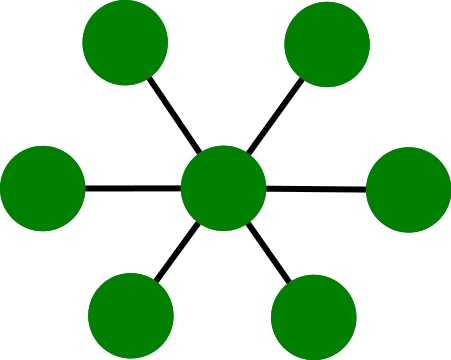
\includegraphics[width=0.6\textwidth]{./imagenes/estrella}
\caption{Topología en estrella} \label{fig:estrella}
\end{figure}

\subsection{Método a utilizar}
\title{Método a utilizar}
Dentro de las \textit{WSN}, podemos elegir entre distintos métodos para realizar la
comunicación entre nuestras motas. Según las necesidades que tenga nuestra red,
utilizaremos uno u otro. Se van a analizar brevemente algunos de los principales:

\begin{description}
  \item[WiFi] \hfill \\
    Basado en el estándar IEEE 802.11. Alta velocidad en transferencia de datos
    (permite adaptación a la velocidad de transmisión) y seguridad en la red pero
    no dispone de mecanismos para ahorrar energía
  \item[Bluetooth] \hfill \\
    Otro estándar de comunicación entre dispositivos. Permite broadcast, una velocidad
    de hasta 24Mbit/s y sus redes son de hasta 8 nodos (uno maestro y siete esclavos).
    En la versión 4 se han introducido métodos para reducir el consumo de energía
  \item[802.15.4] \hfill \\
    Es un estándar propuesto por el IEEE. El ancho de banda es muy pequeño, la latencia
    se sitúa en torno a los 15ms, alcance de entre 10 y 20 metros, permite tener miles
    de nodos en la red, mecanismos para tener un bajísimo consumo de energía y barato
  \item[ZigBee] \hfill \\
    Es un estándar desarrollado sobre 802.15.4, lo que quiere decir que añade capas a la
    propuesta hecha en 802.15.4 (añadiendo algunas funciones)
\end{description}

Todos estos métodos permiten la topología en estrella.\\

Teniendo en cuenta el análisis anterior se concluye que:
\begin{itemize}
  \item WiFi queda descartado: aunque existan redes de sensores que utilicen esta tecnología,
  WiFi no contempla mecanismos para el ahorro de energía. Aunque vaya a ser necesaria una alta velocidad
  (debido a los requisitos temporales del sistema), no hace falta tanta como la que
  proporciona este mecanismo de comunicación (por lo que se vería desperdiciada)
  \item Bluetooth se descarta: a través de la capa de aplicación, algunas implementaciones
  de redes inalámbricas de sensores han conseguido aumentar el número máximo de nodos por red.
  Por otra parte, aunque la versión 4 de Bluetooth esté pensada para economizar el gasto energético,
  este sigue siendo demasiado alto (es algo que cualquier usuario experimenta día a día cuando
  conecta unos auriculares, un manos libres o una smartband a su smartphone, descendiendo el nivel de
  carga de la batería a una velocidad muy alta)
  \item 802.15.4 o ZigBee son la solución: cumplen con casi todos los requisitos.
  El problema que puede presentarse viene dado por las velocidades de transferencia: aunque no
  se necesite realizar grandes traspasos de información, las comunicaciones deben
  hacerse de la manera más rápida posible. Hay que tener en cuenta que ZigBee está construido a partir
  de 802.15.4, lo que significa que la latencia será mayor (habrá que sumar la de 802.15.4 a la que provoquen
  las capas que añade ZigBee). También puede ocurrir que en el canal en el que se estén realizando las comunicaciones
  se esté produciendo otra (en ese caso, la velocidad de transmisión disminuirá)
\end{itemize}

\begin{figure}[htb]
\centering
\captionsetup{justification=centering}
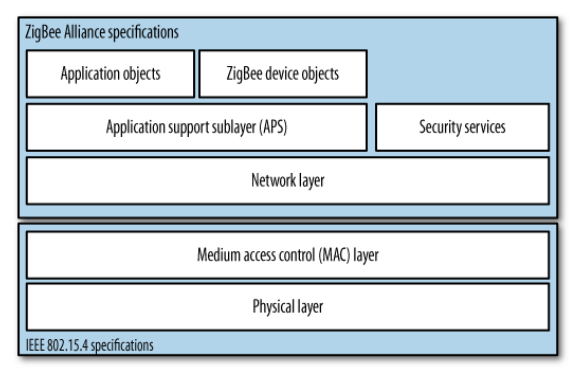
\includegraphics[width=1\textwidth]{./imagenes/zigbeestack}
\caption{ZigBee Stack \\
\scriptsize{Imagen extraída de \cite{faludi} (figura 8.1)} } \label{fig:stackzigbee}
\end{figure}

Finalmente se ha elegido trabajar con ZigBee aunque, probablemente, con 802.15.4 sería suficiente (incluso
mejor al tener una menor latencia). El motivo de esta selección viene determinado porque las motas disponibles
en el laboratorio son de tipo ZigBee, no habiendo de la otra variedad.\\

Para ser más específicos, se va a utilizar el modelo ``XBee 2mW Wire Antenna - Series 2 (ZigBee Mesh)", cuya referencia es
``XB24-Z7WIT-004" (ID: OUR XBEE2 e IC: 4214A-XBEE2) y que es la implementación de la compañía ``Digi" \cite{productdetaildigi}.


\begin{figure}[htb]
\centering
\captionsetup{justification=centering}
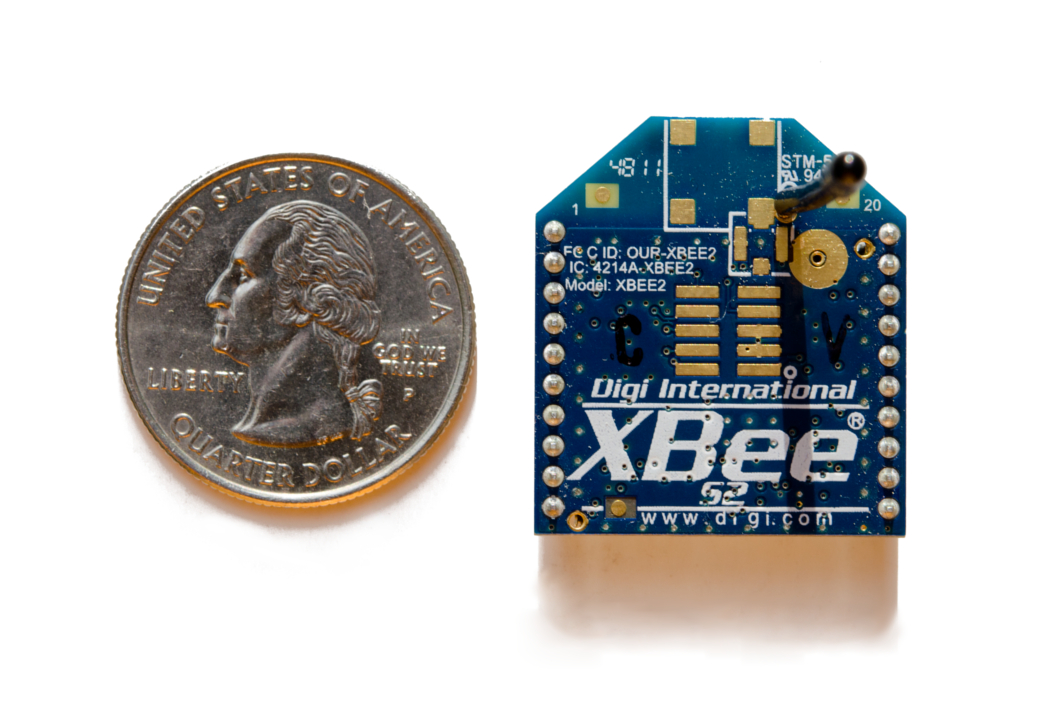
\includegraphics[width=1\textwidth]{./imagenes/xbeequarter}
\caption{Una mota XBee junto a un cuarto de dólar\\
\scriptsize{Imagen extraída de https://en.wikipedia.org/wiki/XBee} } \label{fig:xbeequarter}
\end{figure}

\begin{figure}[htb]
\centering
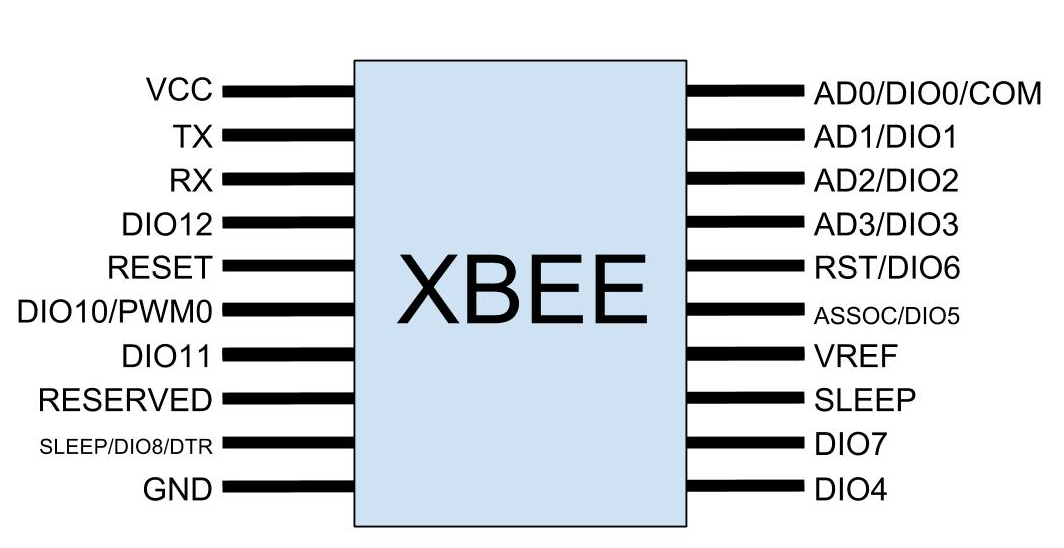
\includegraphics[width=1\textwidth]{./imagenes/xbeepinout}
\caption{XBee PINOUT} \label{fig:xbeepinout}
\end{figure}

En la figura \ref{fig:xbeepinout} podemos ver el esquema de XBee Series 2.

\begin{itemize}
  \item VCC: alimentación
  \item TX: pin de salida de comunicación serial
  \item RX: pin de entrada de comunicación serial
  \item DIO12: entrada o salida digital
  \item Reset: permite resetear el módulo
  \item DIO10/PWM0/RSSI: tiene tres funcionalidades (entrada/salida digital,
    RSSI -”Indicador de Intensidad de la Señal”- o pin de modulación por ancho de pulsos)
  \item DIO11: entrada o salida digital
  \item Reserved: es un pin reservado. No se aconseja conectarlo a nada
  \item SLEEP/DIO8/DTR: también dispone de varias funciones (control de sueño de la mota,
    entrada/salida o señal hardware de handshaking).
  \item GND: tierra
  \item DIO4: entrada o salida digital
  \item DIO7: entrada o salida digital. También puede hacer las funciones de “clear to send”
  \item SLEEP: indicador de sueño. Permite saber si la mota se encuentra durmiendo
    o no (si el estado es alto, se encuentra en funcionamiento)
  \item VFREF: no tiene funcionalidad en este modelo
  \item ASSOC/DIO5: doble función (indicador de pertenencia a red -estado alto si
    está asociada a una red- o entrada/salida digital)
  \item RST/DIO6: doble función (petición de envío o entrada/salida digital)
  \item AD3/DIO3: entrada salida analógica o digital
  \item AD2/DIO2: entrada salida analógica o digital
  \item AD1/DIO1: entrada salida analógica o digital
  \item AD0/DIO0/COM: triple funcionalidad (entrada/salida digital o analógica o puesta en servicio)
\end{itemize}

Sus características técnicas (que se pueden consultar en \cite{xbeedatasheet}) son:
\begin{itemize}
  \item 3.3V @ 40mA
  \item Velocidad máxima: 250kbps
  \item 2mW salida (+3dBm)
  \item 400ft (120m) rango
  \item Antena incorporada
  \item Certificado por FCC
  \item 6 10-bit ADC pines de entrada
  \item 8 pines digitales de entrada/salida
  \item 128-bit encriptación
  \item Modo AT o API
\end{itemize}

En este último punto se nos hablan de dos modos de funcionamiento:

\begin{description}
  \item[AT] \hfill \\
    Es el modo transparente. Una vez establecida la configuración (mediante comandos
    que se envían al dispositivo a través de serial), el dispositivo solo es capaz de
    comunicarse con la mota cuya dirección MAC corresponde con la de la configuración
    (también pueden enviarse paquetes a todos los dispositivos en caso que la dirección
    que se haya configurado sea la de broadcast). Esto quiere decir que, en caso que
    deseemos cambiar el destino de nuestras comunicaciones, tendremos que reconfigurar
    la mota (ya sea enviando comandos AT o utilizando algún software que los envíe
    por nosotros) Es el modo más simple de trabajar con XBee.
 \item[API] \hfill \\
    Este modo permite mucho más. Capacita al desarrollador a:
      \begin{itemize}
        \item Obtener RSSI (fortaleza de la señal respecto a otro dispositivo),
        \item Enviar paquetes a múltiples destinos
        \item Recibir paquetes de distintos tipos
        \item Activar funciones de integridad de datos, recibir ACK...
        \item Conocer el estado de la red
      \end{itemize}
\end{description}



\subsection{Modo API}
\title{Modo API}

Mientras que en el modo transparente los caracteres que escribamos en el puerto
serial de XBee serán enviados directamente a la mota destino, en este modo las
comunicaciones se realizan enviando paquetes con una estructura predefinida.\\

Existen dos formas de comunicarse con la mota cuando se encuentra en este modo:
\begin{itemize}
  \item Pines de entrada/salida: en el caso de querer dar una salida, la deberemos preestablecer en la configuración.
  Un pin que se configure en modo entrada, tomará el valor que le llegue y la mota enviará el valor a la mota destino.
  La propia mota genera el paquete y lo envía.
  \item Puerto serial: permite la creación y envío de distintos tipos de paquetes.
  Esto se hace de forma manual, es decir, se precisa de un controlador que escriba los valores en el puerto serial de XBee.
\end{itemize}

Cada paquete que envía (o recibe) un dispositivo XBee, tiene la estructura de la figura \ref{fig:tramaapi}.

\begin{figure}[htb]
\centering
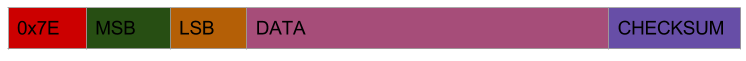
\includegraphics[width=1\textwidth]{./imagenes/tramaapi}
\caption{Paquete XBee en modo API} \label{fig:tramaapi}
\end{figure}

\begin{itemize}
  \item 0x7E: comienzo de la trama
  \item MSB: byte más significativo para la traza
  \item LSB: byte menos significativo para la traza
  \item DATA: puede incluir varias cosas, como el tipo de comando API o AT que se está enviando, parámetros… (para conocer más, )
  \item CHECKSUM: checksum de la trama
\end{itemize}

Para generar estas tramas utilizaremos una biblioteca open source que se encuentra en GitHub (\cite{libraryArduinoXBee}).
Gracias a ella, no tendremos que preocuparnos de generar los distintos elementos del paquete
(como el delimitador de comienzo o el cálculo del checksum).\\

Para conocer más sobre el modo API, el lector puede consultar el capítulo 5 (\textit{API and a Sensor Network}) de \cite{faludi}.\\

\subsection{XCTU: el software para manipular las motas}
\title{XCTU: el software para manipular las motas}
\label{xctu}
Este software es distribuido gratuitamente por Digi \cite{licenciaXCTU} y se puede descargar desde la página oficial
de dicha empresa.

Para conectar XBee a nuestro ordenador, debemos conectar las patillas de XBee del puerto serial a un
FTDI (por ejemplo) y con una conexión serial o USB, a nuestro ordenador. Otra posibilidad es obtener
una placa ``XBee Explorer" como la de la figura \ref{fig:xbeeexplorer}.


\begin{figure}[htb]
\centering
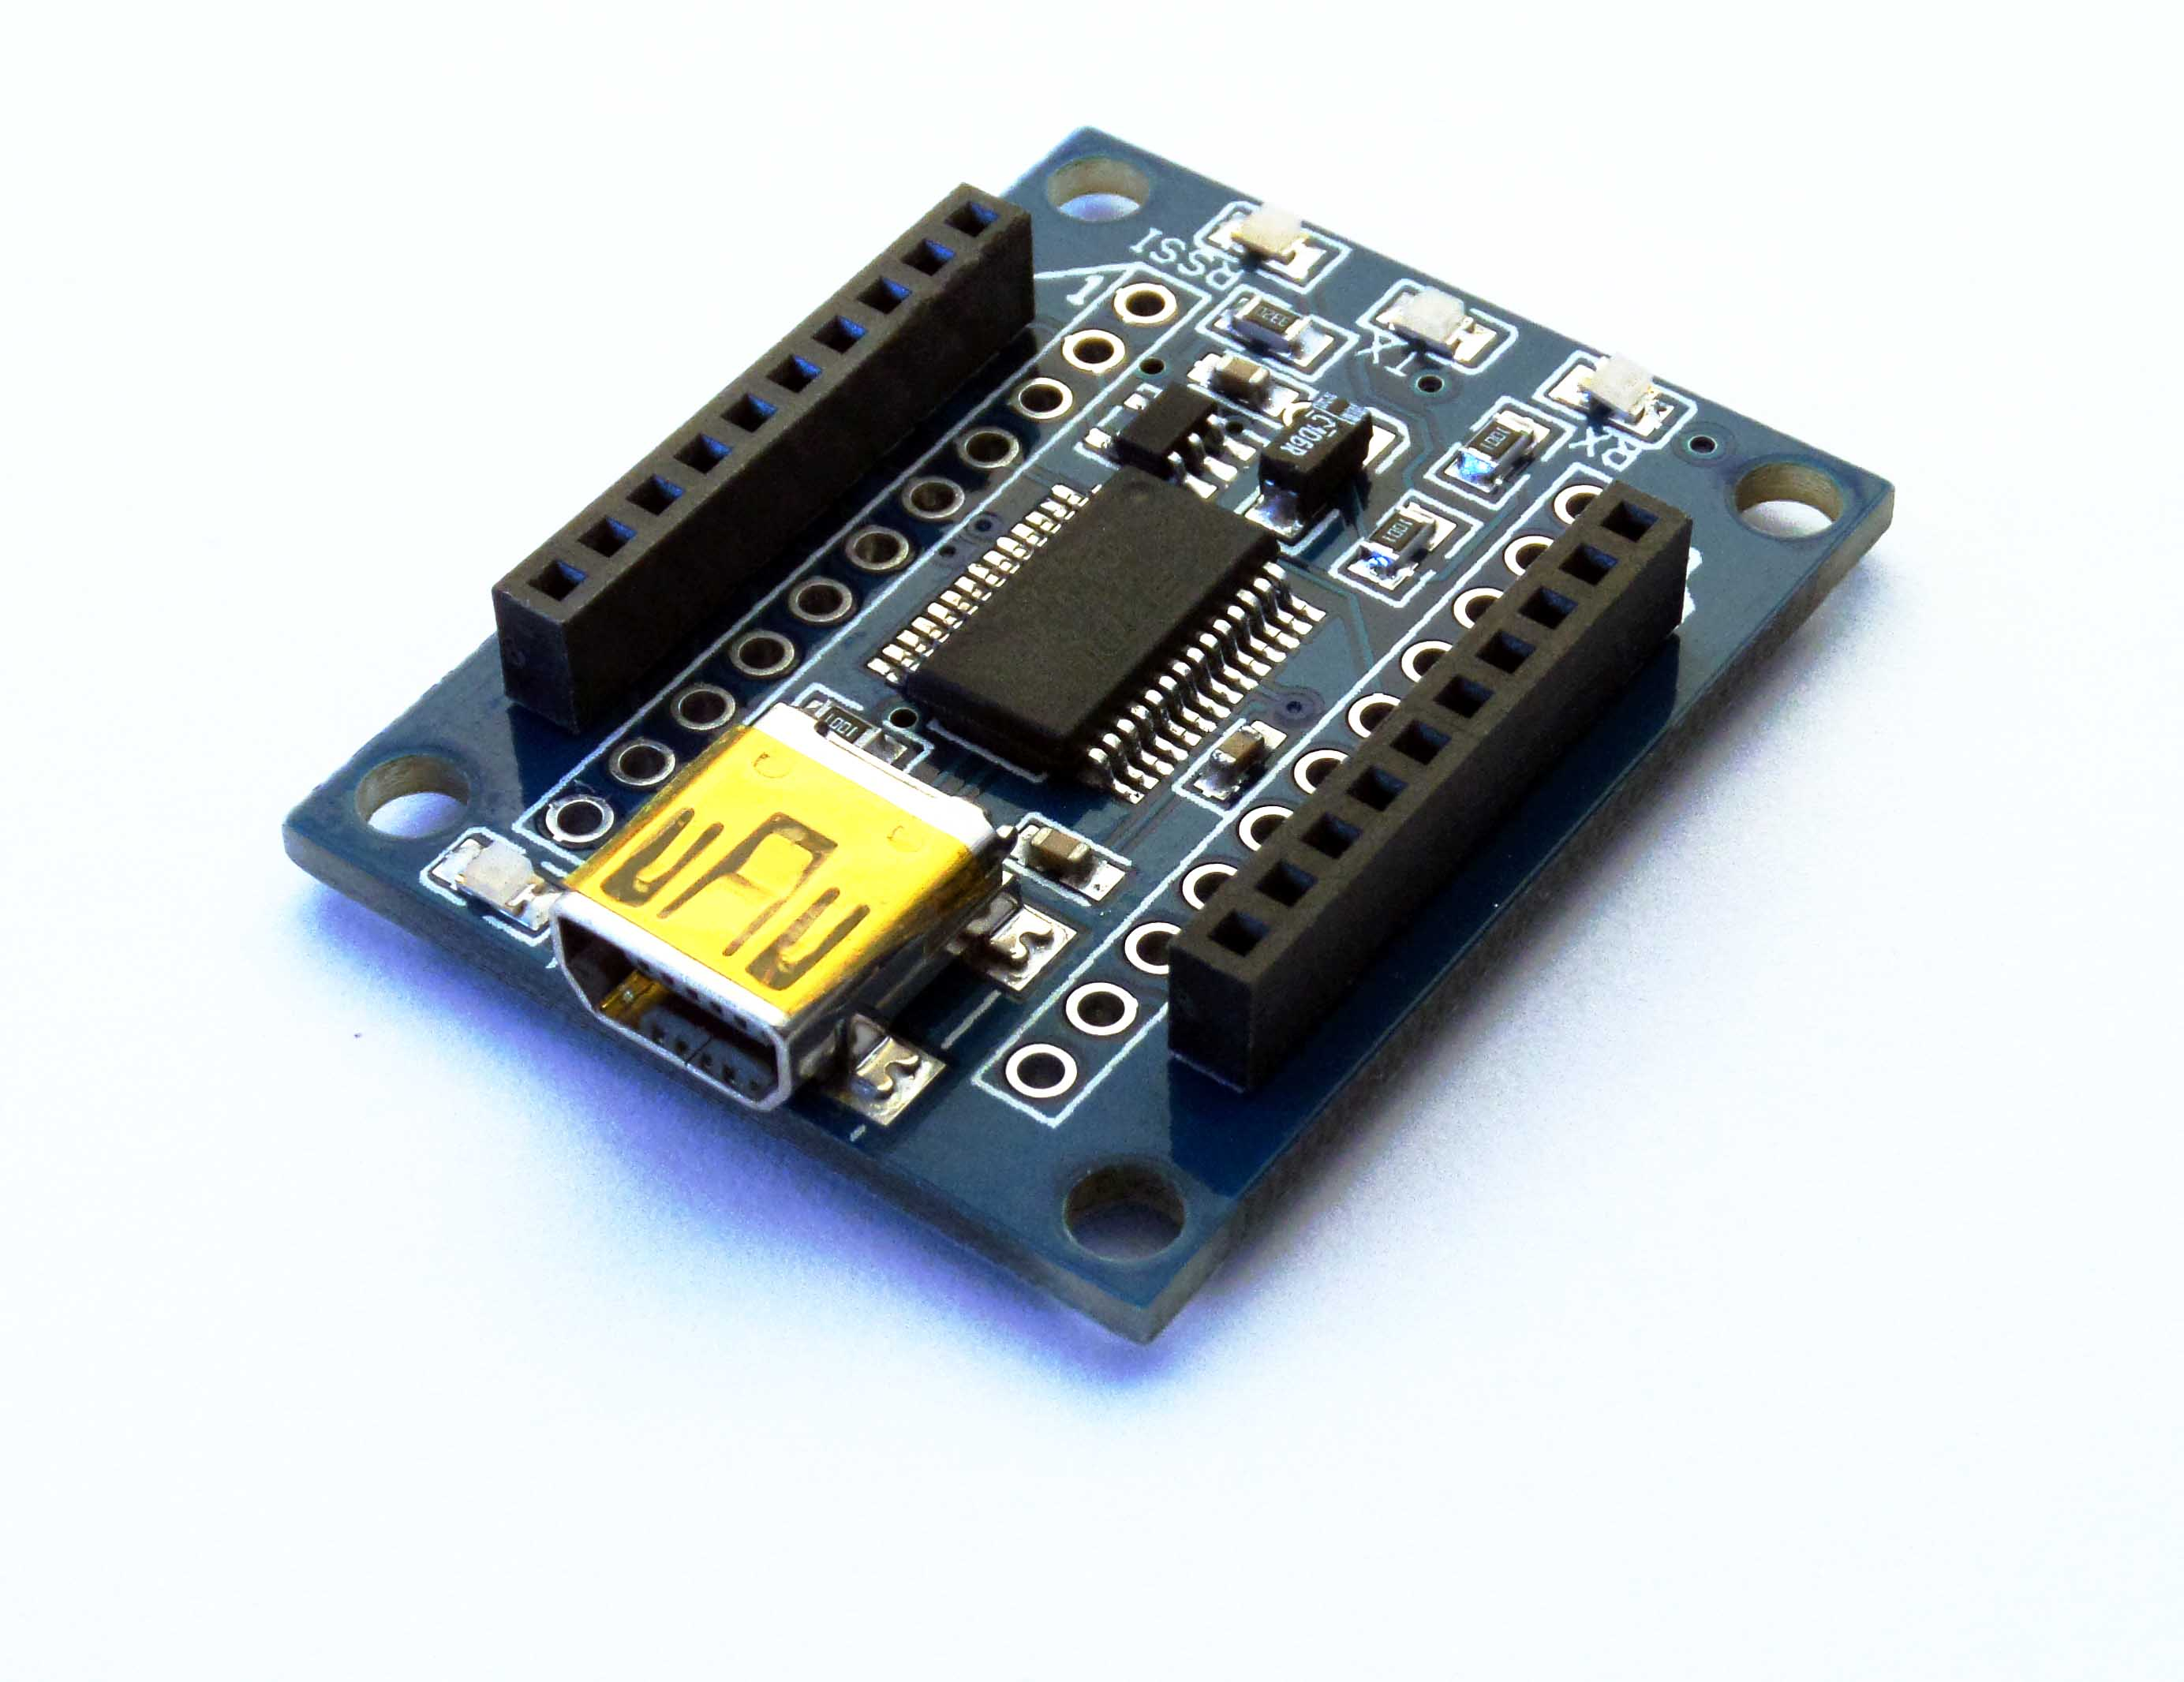
\includegraphics[width=0.8\textwidth]{./imagenes/xbeeexplorer}
\caption{XBee USB Explorer. Imagen extraída de \scriptsize{http://xbee.cl/xbee-explorer-usb/}} \label{fig:xbeeexplorer}
\end{figure}


En la ventana principal tenemos tres secciones: a la izquierda, la lista de los dispositivos
que tenemos conectados a nuestro ordenador; a la derecha, un panel de administración que variará
en función de lo que estemos haciendo con la mota; y arriba, las opciones relacionadas con el descubrimiento
de nuevos dispositivos (izquierda) o distintas acciones sobre la mota (derecha). Podemos verlo en la figura \ref{fig:interfaz1}.\\

\begin{figure}[!htb]
\centering
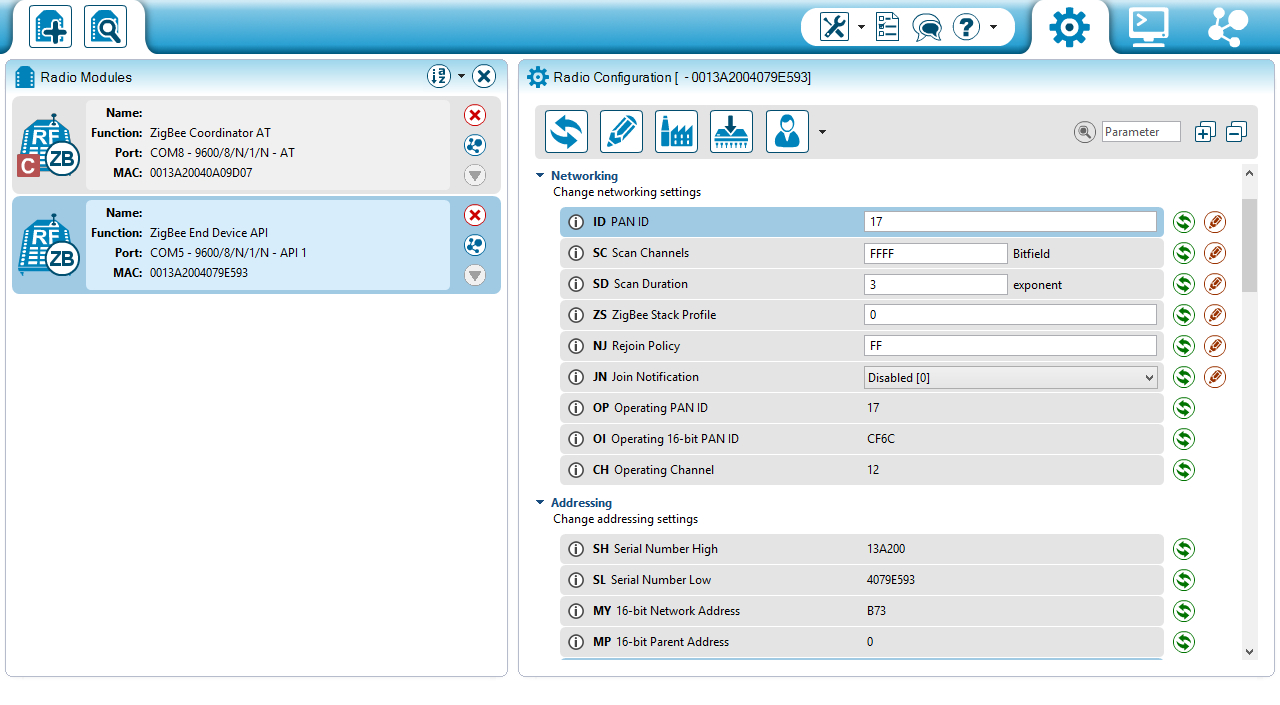
\includegraphics[width=1\textwidth]{./imagenes/interfaz1}
\caption{Interfaz XCTU} \label{fig:interfaz1}
\end{figure}

Lo primero que tendremos que hacer una vez hayamos conectado nuestra mota al ordenador, será descubrirla con XCTU
utilizando una de las dos opciones que tenemos arriba a la izquierda (es importante mencionar que, en caso que se nos
pida resetear la mota y, como es el caso de nuestro modelo, no tengamos un botón para resetear, deberemos unir con un
cable la patilla \guillemotleft RST\guillemotright con \guillemotleft GND\guillemotright).\\

\begin{figure}[!htb]
\centering
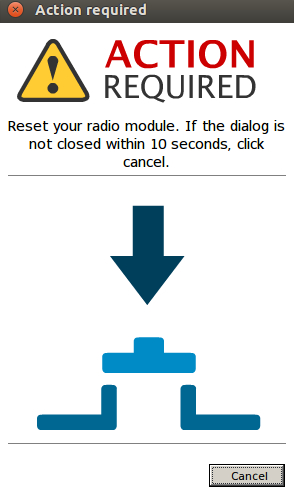
\includegraphics[width=0.5\textwidth]{./imagenes/xctureset}
\caption{Paquete XBee en modo API} \label{fig:xctureset}
\end{figure}

Una vez que tengamos la mota descubierta tendremos el menú de configuración (el de la rueda dentada) abierto. En él podremos
cambiar el firmware, volver a los ajustes de fábrica, establecer un nombre para la mota, ver la dirección de destino,
\textit{PAN} (Personal Area Network) a la que unirse... en función del firmware que tenga instalado la mota, habrá unas opciones u otras
(por ejemplo, en caso de tener un dispositivo final, podremos configurar cada cuánto tiempo de inactividad puede el nodo
entrar en suspensión).\\

En el siguiente menú, podremos ver qué es lo que está recibiendo (o enviando) nuestro XBee.
Se monitoriza el puerto serial (ver figura \ref{fig:interfaz2}).\\

\begin{figure}[!htb]
\centering
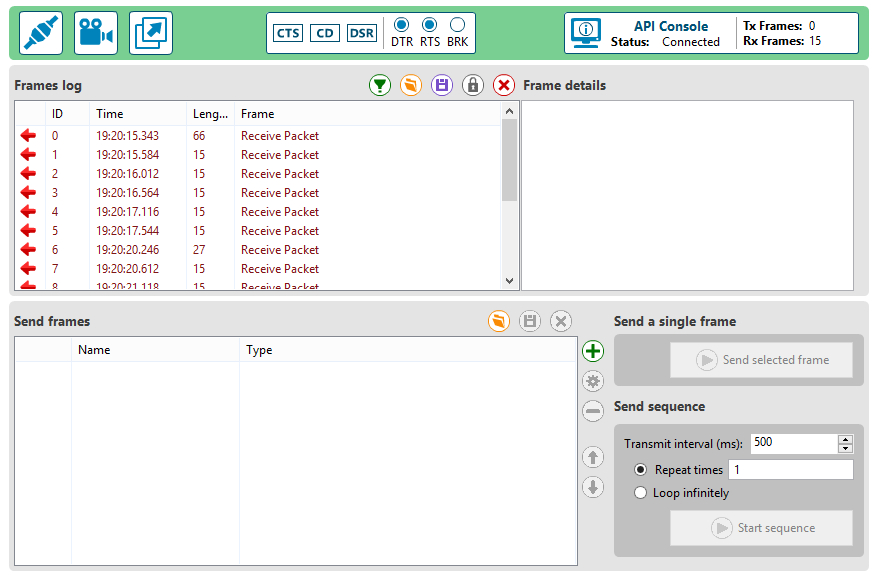
\includegraphics[width=1\textwidth]{./imagenes/interfaz2}
\caption{Monitorizando el puerto serial (modo API) en XCTU} \label{fig:interfaz2}
\end{figure}

Finalmente el tercer menú nos brinda algunas opciones relacionadas con la nube de Digi y la posibilidad
de conocer qué nodos están interconectados en la red (solo disponible si el módulo está en modo API).\\

\subsection{Posible problema de escalabilidad}
\title{Posible problema de escalabilidad}

Aunque estas redes están pensadas para contar con miles de dispositivos,
estas suelen estar formadas por un coordinador y varios routers.
Al haber solamente un coordinador, es éste quien debe almacenar
toda la información que concierne a la red.\\

La dirección MAC de una mota se divide en dos partes iguales (dirección alta y dirección baja).
Teniendo en cuenta que la MAC tiene un tamaño de 64 bits, cada parte tiene un total de 32 bits.
La dirección alta es la misma para todos los nodos y la baja es la que cambia. Por tanto, tendremos 2\textsuperscript{32} direcciones
disponibles (más de 4.000.000.000) o lo que es lo mismo, podremos direccionar hasta 2\textsuperscript{32} dispositivos.\\

El problema que se presenta es el siguiente: Cada dirección ocupa 64 bits, osea, 8 bytes. Si deseamos guardar 150
direcciones (en la introducción se hablaba de casos en los que había bandas que superan los 100 integrantes por lo que
deberíamos pensar en guardar un número mayor de direcciones, donde cada dirección sería un músico), tendremos que almacenar
1.200 bytes (8 bytes x 150 direcciones), unos 1.17KB. Si la memoria destinada a direcciones en la mota es menor que este tamaño,
pueden producirse problemas.\\

Ya que no se disponen de tantos dispositivos para hacer un experimento ni se ha encontrado información al respecto,
no podemos predecir el comportamiento del sistema ante tal número de nodos.\\

\section{Controlador}
\title{Controlador}

Para llevar a cabo el control de los componentes es necesario algún tipo de microcontrolador
o placa controladora. Se han estudiado dos posibles soluciones:

\begin{description}
  \item[PIC] \hfill \\
    \begin{itemize}
      \item Son microcontroladores
      \item Precio muy bajo
      \item Gran variedad
      \item Pequeño tamaño
      \item Programación en ensamblador, con una media de 35 instrucciones
      \item Simples pero orientados a un público muy relacionado con la programación
    \end{itemize}
    \begin{figure}[!htb]
    \centering
    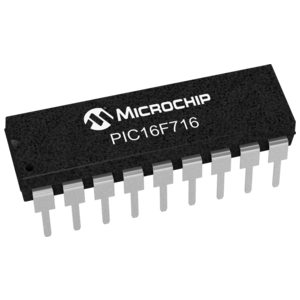
\includegraphics[width=0.5\textwidth]{./imagenes/pic}
    \caption{PIC16F716\\  \scriptsize{Imagen extraída de http://www.microchip.com/}} \label{fig:pic}
    \end{figure}
  \item[Arduino] \hfill \\
    \begin{itemize}
      \item Placa con un microcontrolador
      \item Programación en alto nivel (Python, Scratch, JavaScript o un derivado de Processing)
      \item Muchas bibliotecas para extender funcionalidad
      \item Existe una versión Wear (Arduino Lilypad, mostrado en la figura \ref{fig:lilypad})
      \item Shields para XBee (como la que se muestra en la figura \ref{fig:lilypadxbee})
    \end{itemize}
    \begin{figure}[!htb]
    \centering
    \captionsetup{justification=centering}
    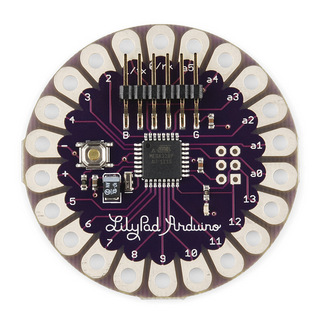
\includegraphics[width=0.5\textwidth]{./imagenes/lilypad}
    \caption{Arduino Lilypad\\
     \scriptsize{Imagen extraída de https://www.arduino.cc}} \label{fig:lilypad}
    \end{figure}

    \begin{figure}[htb]
    \centering
    \captionsetup{justification=centering}
    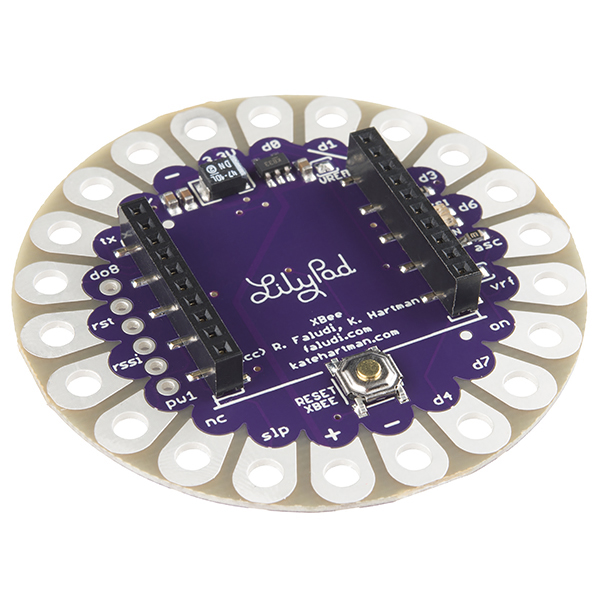
\includegraphics[width=0.5\textwidth]{./imagenes/lilypadxbee}
    \caption{Shield XBee Lilypad\\
      \scriptsize{Imagen extraída de https://www.faludi.com/ \cite{faludi}}} \label{fig:lilypadxbee}
    \end{figure}
\end{description}


\clearpage

Sabiendo que Arduino se encuentra orientado a un público con una menor formación en electrónica y
programación (por lo tanto, accesible a una mayor comunidad), se adecua más al objetivo de este proyecto.
También hay que tener en cuenta la cantidad de bibliotecas
existentes en Arduino (lo que nos ayudará a abstraernos de algunas tareas). Por contra,
PIC es más competitivo en tamaño y precio.\\

\subsection{IDE Arduino}
\title{IDE Arduino}

El IDE de Arduino puede ser descargado de su página oficial \cite{arduinoWeb}. Es de código abierto y se
encuentra basado, igual que el lenguaje que se utiliza, en Processing (un lenguaje basado a su vez en Java y C).

En el menú superior tenemos acceso a distintas opciones como guardar nuestro proyecto, cargar un proyecto de ejemplo,
instalar nuevas bibliotecas, seleccionar la placa para la que estamos desarrollando, el puerto en el que se encuentra dicha
placa...\\

\begin{figure}[!htb]
\centering
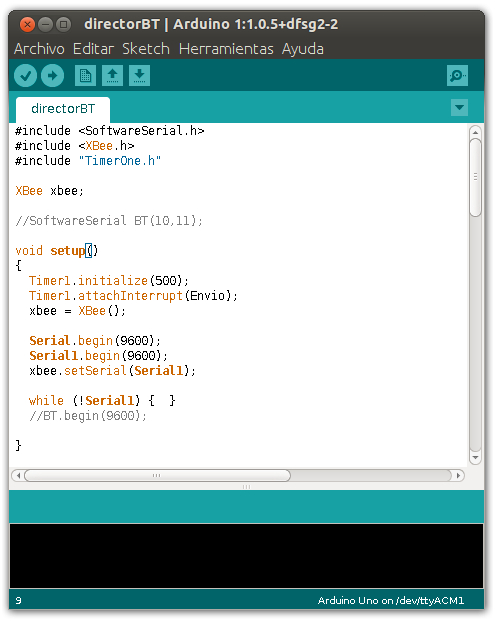
\includegraphics[width=0.6\textwidth]{./imagenes/arduinoide}
\caption{IDE Arduino} \label{fig:arduinoide}
\end{figure}


Justo debajo tenemos una serie de opciones (``Verificar", que compilará nuestro código; ``Cargar", que lo
subirá a nuestra placa Arduino; ``Nuevo", que creará un nuevo proyecto Arduino; ``Abrir", permite abrir un proyecto
Arduino ya cread; ``Guardar", para guardar el actual proyecto). A la derecha del todo, tenemos un monitor para el
puerto serial (para poder acceder a la comunicación entre nuestro equipo y la placa Arduino).\\

Si el lector no está familiarizado con el entorno y desea conocerlo algo más, puede consultar la bibliografía \cite{arduinoInicia} y
\cite{arduino24}.


\section{Actuador}
\title{Actuador}
Para que el músico sepa qué pulso es el correcto necesita alguna señal. Para ello
se ha decidido utilizar un micromotor vibrador. Para ser más exactos, el modelo 310-101 de la empresa
``Precision Microdrives" (figura \ref{fig:micromotor}).\\

\begin{figure}[!htb]
\centering
\captionsetup{justification=centering}
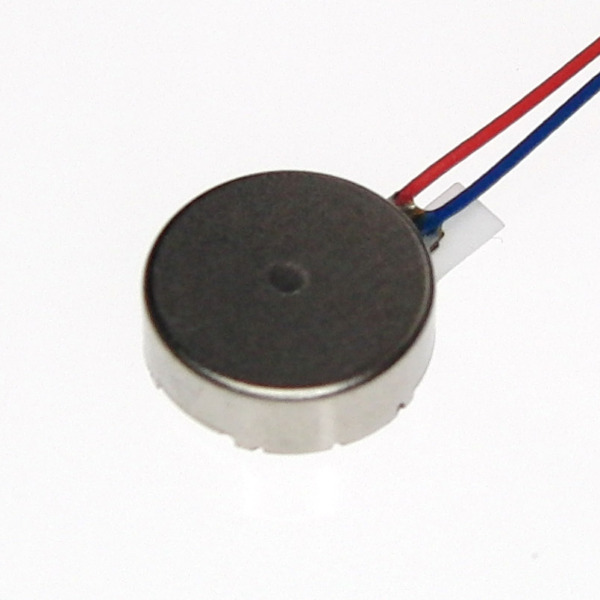
\includegraphics[width=0.5\textwidth]{./imagenes/micromotor}
\caption{Micromotor 310-101\\
\scriptsize{Imagen extraída de https://catalog.precisionmicrodrives.com}} \label{fig:micromotor}
\end{figure}


Sus características técnicas son:

\begin{itemize}
  \item Voltaje: 3V
  \item Diámetro: 10mm
  \item Longitud del cuerpo 3.4mm
  \item Peso: 1.2g
  \item Velocidad: 12000 rpm
  \item Intensidad: 85mA
  \item Resistencia: 75 Ohm
  \item Amplitud de vibración: 0,8G
\end{itemize}

Se puede consultar su datasheet en la bibliografía \cite{micromotorData}.



\section{Alimentación}
\title{Alimentación}

Gracias a la existencia de distintos tipos de placas Arduino, podemos crear dispositivos
con una forma u otra (como otro de los objetivos es la posibilidad de aumentar la funcionalidad
el sistema, habrá funcionalidades que necesiten de placas Arduino con un número distinto de
entradas/salidas al que se utilice aquí), aunque tendremos que intentar que sea lo más compacto
posible (para no ignorar aquel objetivo en el que se deseaba crear un sistema pequeño y discreto).\\

Por ejemplo, en caso que nos encontremos utilizando un Arduino Lilypad, la versión vestible de Arduino,
podremos elegir alguna de las opciones que se nos brindan para alimentar nuestro circuito, como el “LLYP-PSU”,
en el que podremos colocar una pila AAA o el “LilyPad 20mm Coin Cell Battery Holder”, para pilas de botón (cuyos
planos se encuentran disponibles en GitHub \cite{lilypadcoin}).\\

Otra opción a contemplar (y que cobrará mayor sentido al no usar la versión de Arduino vestible)
es la de utilizar bancos de energía (baterías externas). Estas baterías están pensadas para cargar
dispositivos móviles con gran consumo energético. La alta capacidad de estas baterías y el bajo consumo
de Arduino y XBee, tendrá como resultado la despreocupación del usuario en cuanto al plano energético.\\

Como se ha mencionado, en función del tipo de Arduino con el que construyamos nuestro ArduBand,
se seleccionará un tipo de alimentación u otra, quedando esto, generalmente, a opción del usuario
(sobre todo en el caso de la batería externa).\\

\section{Comunicación uno a muchos: estudio preliminar}
\title{Comunicación uno a muchos: estudio preliminar}

En los capítulos de \ref{cap:Diseno} y \ref{cap:Analisis} se ha ido viendo que es necesario
que un dispositivo emita un mensaje al resto de nodos de la red. Teniendo en cuenta que el
sistema se va a implementar como una red, la solución técnica que parece más adecuada
es realizar un \textit{broadcast} (un nodo envía una trama de datos a una dirección
especial, llamada dirección de broadcast, y todos los nodos reciben la trama de datos). Al querer
realizar una red con topología de estrella, es claro que el dispositivo central de
la red, y que interconecta al resto, será el que haga las veces de emisor.\\

ZigBee como tal permite conectar en estrella, malla o árbol. Según \cite{faludi} (tabla 1.1), se
puede configurar el XBee Series 2 (el que se está utilizando) para utilizar cualquiera de estar
topologías por defecto. Sin embargo no hay documentación sobre la forma de cambiar el comportamiento
por defecto (red de tipo malla).

En las redes formadas por dispositivos XBee tenemos tres tipos de dispositivos:
\begin{itemize}
  \item Coordinador: debe existir, al menos, uno por red. En caso de haber más, solo uno
  toma este rol (en caso de haber más de uno, se ponen de acuerdo y solo uno de ellos toma
  este rol, mientras que el otro pasa a ejercer de router). Se encarga de dirigir la red,
  estableciendo las rutas que deben seguir los paquetes. Puede comunicarse con todos los nodos
  \item Router: permite conectar nodos finales u otros routers con el coordinador. Puede
  comunicarse solo con el nodo coordinador (y sirve como puente para el traspaso de información
  entre el nodo coordinador y un nodo cualquiera)
  \item Dispositivo final: solo puede enviar información al coordinador (pudiendo utilizar
  los routers para hacer llegar la trama hasta su destino). Pasan la mayor parte del tiempo
  durmiendo, es decir, en un estado de bajo consumo energético
\end{itemize}

\begin{figure}[!htb]
\centering
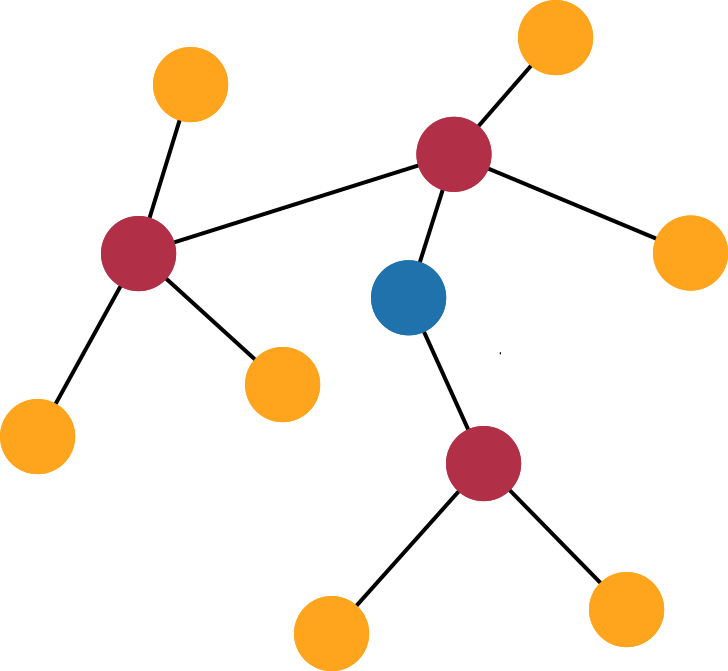
\includegraphics[width=0.6\textwidth]{./imagenes/mesh}
\caption{Red de tipo \textit{mesh}} \label{fig:mesh}
\end{figure}

En la figura \ref{fig:mesh} podemos ver un ejemplo de red XBee ZigBee.
\begin{itemize}
  \item  \textcolor{blueS}{$\blacksquare$} Coordinador
  \item  \textcolor{rojoOscuroS}{$\blacksquare$} Router
  \item  \textcolor{naranjaS}{$\blacksquare$} Dispositivo final
\end{itemize}

Teniendo en cuenta los tipos de nodos que tenemos, podemos crear una topología en estrella
(la que más encaja con nuestro proyecto) a partir de la topología en malla: no tendremos
disposivios de tipo router. De esta forma evitaremos que haya saltos intermedios entre
el dispositivo final (músico) y el director.\\

Esto puede parecer un inconveniente en bandas largas (no disponemos de routers
que hagan de puente con dispositivos finales que se encuentren demasiado lejos)
pero si volvemos a mirar la tabla 1.1 de \cite{faludi}, veremos que el rango
de alcance se sitúa entre los 40 y 120 metros. Teniendo en cuenta que en la
formación de una banda de música la separación entre dos filas de músicos es de
1 metro aproximadamente, en el peor de los casos, estaríamos llegando a 80 metros
(si situamos el dispositivo en el centro de la banda). Si establecemos una media de
4 músicos por fila, en una banda de 80 metros de largo tendríamos 320 músicos.
Teniendo en cuenta que la banda de la que se hablaba en la introducción \cite{cigarreras}
es una de las más numerosas con alrededor de 140 músicos, es claro que esto no es
un problema.\\

\subsection{Problema en broadcast}
\title{Problema en broadcast}
\label{subsec:problemabroadcast}

En el apartado anterior se explicaba que la solución que parece más directa es realizar
un \textit{broadcast}. Pero es una idea que se desecha rápidamente al hacer el siguiente experimento:

\begin{enumerate}
  \item Se configura una mota como coordinador (instalándo el firmware oportuno, eligiendo el modo API)
  \item A esta mota se le inserta la dirección de \textit{broadcast} como
  dirección de destino (0x0 para la DH y 0xFFFF para DL)
  \item Se le inserta un \textit{PAN ID}
  \item Se configura otra mota como dispositivo final (con firmware en modo API
  y con el mismo \textit{PAN ID})
  \item Pulsamos sobre el menú para controlar el puerto serial (en la mota coordinadora)
  (la descrita en la figgura \ref{fig:interfaz2})
  \item Creamos un paquete con un solo carácter y ponemos que se envíe infinitas veces
  cada 500ms
  \item Comprobamos, en el dispositivo final, la traza y comprobamos lo tiempos
\end{enumerate}

El configurar ambas motas en modo API es por los siguientes motivos:
\begin{itemize}
  \item Nodo final: XCTU muestra el tiempo de llegada de los paquetes. En modo AT
    (transparente), no
  \item Nodo director: para poder modificar los datos del paquete
\end{itemize}

Este experimento se ha realizado varias veces. Un ejemplo de lo que ocurre se muestra
en la figura \ref{fig:pruebasxctu_broadcast}. En la figura \ref{fig:graficabroadcast}
se muestra de una forma distinta la misma información (el eje X está en segundos y en
el eje Y se muestra la llegada de un paquete).\\

\begin{figure}[!htb]
\centering
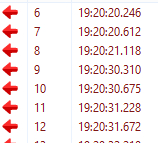
\includegraphics[width=0.4\textwidth]{./imagenes/pruebasxctu_broadcast}
\caption{Traza temporal de llegada de paquetes en X-CTU con \textit{broadcast}} \label{fig:pruebasxctu_broadcast}
\end{figure}


\begin{figure}[!htb]
\centering
\captionsetup{justification=centering}
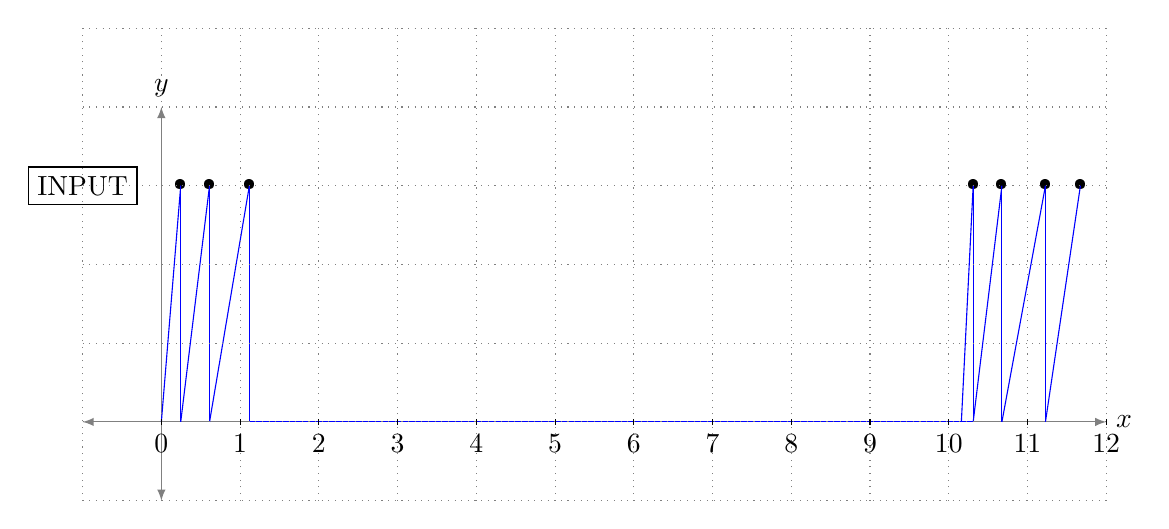
\begin{tikzpicture}
\draw[latex-latex, thin, draw=gray] (-1,0)--(12,0) node [right] {$x$};
\draw[latex-latex, thin, draw=gray] (0,-1)--(0,4) node [above] {$y$};

\foreach \Point in { (0.246,3),(0.612,3),(1.118,3),(10.310,3),(10.675,3),(11.228,3),(11.672,3) }{
   \node at \Point {\textbullet};
}

\draw [blue,solid] (0,0) -- (0.246,3);
\draw [blue,solid] (0.246,3) -- (0.246,0);
\draw [blue,solid] (0.246,0) -- (0.612,3);
\draw [blue,solid] (0.612,3) -- (0.612,0);
\draw [blue,solid] (0.612,0) -- (1.118,3);
\draw [blue,solid] (1.118,3) -- (1.118,0);
\draw [blue,solid] (1.118,0) -- (10.310,0);
\draw [blue,solid] (10.160,0) -- (10.310,3);
\draw [blue,solid] (10.310,3) -- (10.310,0);
\draw [blue,solid] (10.310,0) -- (10.675,3);
\draw [blue,solid] (10.675,3) -- (10.675,0);
\draw [blue,solid] (10.675,0) -- (11.228,3);
\draw [blue,solid] (11.228,3) -- (11.228,0);
\draw [blue,solid] (11.228,0) -- (11.672,3);

\draw [dotted, gray] (-1,-1) grid (12,5);

\foreach \x in {0,1,2,3,4,5,6,7,8,9,10,11,12}
    \draw (\x cm,1pt) -- (\x cm,-1pt) node[anchor=north] {$\x$};

\node[draw] at (-1,3) {INPUT};
\end{tikzpicture}


\caption{Representación temporal de la llegada de paquetes utilizando \textit{broadcast}\\
 (X está en segundos)} \label{fig:graficabroadcast}
\end{figure}

Aunque parece al principio que la recepción de paquetes es regular, después hay un largo
periodo de tiempo (unos 9 segundos) donde no se recibe nada.\\

Si modificamos el paquete en el nodo director para que no envíe ACK de la capa de
aplicación (que podría ser el culpable), se obtienen similares resultados. Para modificar el paquete simplemente
hay que crearlo de la misma forma que antes y, en el editor de paquetes que provee XCTU
(en el mismo lugar donde se crean), se cambia el segundo \textit{byte} de la traza por 0. Si
por ejemplo tenemos el siguiente paquete:  \texttt{7E 01 0F 90 00 7D 33 A2 00 40 A0 9B EC 00 00 01 78 DC},
deberemos convertirlo en este otro  \texttt{7E 00 0F 90 00 7D 33 A2 00 40 A0 9B EC 00 00 01 78 DC}
(solo cambia el segundo \textit{byte}).

Este problema podríamos achacarlo a la capa firmware de la mota (que podría contener mecanismos
para comprobar la integridad de los paquetes y evitar que lleguen trazas corruptas).
Sin embargo, es demasiado tiempo como para que este sea el problema (además, en una comunicación \text{unicast}
(con un solo nodo), el problema no existe -como podemos ver en la figura \ref{fig:xctu_comunicacionunoauno}- y en la gráfica
\ref{fig:graficaunicast}, ya que la tasa de llegada de paquetes se mantiene constante -aproximadamente-).

\begin{figure}[!htb]
\centering
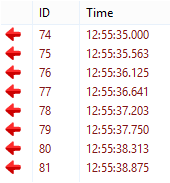
\includegraphics[width=0.4\textwidth]{./imagenes/xctu_comunicacionunoauno}
\caption{Traza temporal de llegada de paquetes en X-CTU con \textit{unicast}} \label{fig:xctu_comunicacionunoauno}
\end{figure}


\begin{figure}[!htb]
\centering
\captionsetup{justification=centering}
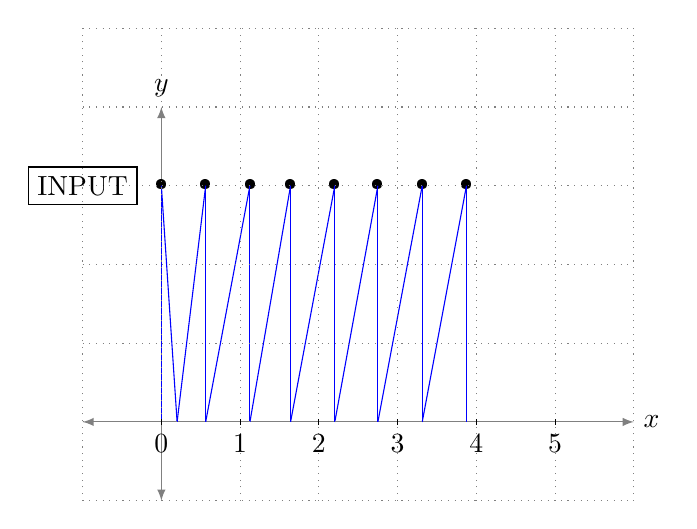
\begin{tikzpicture}
\draw[latex-latex, thin, draw=gray] (-1,0)--(6,0) node [right] {$x$};
\draw[latex-latex, thin, draw=gray] (0,-1)--(0,4) node [above] {$y$};

\foreach \Point in { (0,3),(0.563,3),(1.125,3),(1.641,3),(2.203,3),(2.750,3),(3.313,3),(3.875,3) }{
   \node at \Point {\textbullet};
}

\draw [blue,solid] (0,0) -- (0,3);
\draw [blue,solid] (0,3) -- (0.2,0);
\draw [blue,solid] (0.2,0) -- (0.563,3);
\draw [blue,solid] (0.563,3) -- (0.563,0);
\draw [blue,solid] (0.563,0) -- (1.125,3);
\draw [blue,solid] (1.125,3) -- (1.125,0);
\draw [blue,solid] (1.125,0) -- (1.641,3);
\draw [blue,solid] (1.641,3) -- (1.641,0);
\draw [blue,solid] (1.641,0) -- (2.203,3);
\draw [blue,solid] (2.203,3) -- (2.203,0);
\draw [blue,solid] (2.203,0) -- (2.750,3);
\draw [blue,solid] (2.750,3) -- (2.750,0);
\draw [blue,solid] (2.750,0) -- (3.313,3);
\draw [blue,solid] (3.313,3) -- (3.313,0);
\draw [blue,solid] (3.313,0) -- (3.875,3);
\draw [blue,solid] (3.875,3) -- (3.875,0);

\draw [dotted, gray] (-1,-1) grid (6,5);

\foreach \x in {0,1,2,3,4,5}
    \draw (\x cm,1pt) -- (\x cm,-1pt) node[anchor=north] {$\x$};

\node[draw] at (-1,3) {INPUT};
\end{tikzpicture}

\caption{Representación temporal de la llegada de paquetes utilizando \textit{unicast}\\
(X está en segundos)} \label{fig:graficaunicast}
\end{figure}

Cabe destacar que se recibe un paquete más en menos tiempo.\\

El problema viene por la forma en la que está implementado el \textit{broadcast}:
los nodos se encuentran en una topología de malla y, cada vez que reciben un broadcast,
lo repiten hasta tres veces. Esto no sería un problema si no fuera por que la red
permite un número máximo de broadcast a la vez. Al llegar a ese límite, la mota
coordinadora deja de poder seguir enviando paquetes (no solo hasta que terminen los
\textit{broadcast} existentes, sino hasta que cada mota termine de reenviar 3 veces
cada uno de los paquetes que ha recibido). Es por eso que ha tenido que pasar un tiempo
hasta que la red se sature. Si esto ha pasado con un solo nodo receptor, el problema
se agravaría cuanto mayor fuese la cantidad de nodos en la red. \\

En otras versiones de la mota existe la posibilidad de crear un \textit{multicast},
pero no en esta, por lo que no es una solución viable.\\

La solución que se propone es enviar individualmente a cada dispositivo el paquete, es decir,
hacer un \textit{broadcast} a base de \textit{unicast}. Facilitar esta tarea, es mejor
utilizar el modo API (en el modo AT se puede, pero habría que estar entrando constantemente
al modo comando y, a veces, cuando se entra en este modo, la mota necesita ser reinicia -y,
al no poder reiniciarla, dejaría de funcionar ese nodo-.)\\

Nace ahora una nueva contrariedad: existe un retardo inevitable (de unos pocos milisegundos)
cada vez que se envía un paquete. Entre dos envíos no es problema ya que, cuando
se sincronicen los nodos, los músicos no notarán diferencia. Cuando se envíen 50, sí lo será.\\

Supongamos que hay 50 músicos y cada envío produce un retardo de 15ms. Cuando se llegue al músico
50, habrá habido 49 envíos, luego:
\[
  49 \times 15 = 735ms
\]

Es un retardo de casi un segundo. Como remedio, se propone lo siguiente: en vez de
sincronizar siempre todos los nodos, se sincronizan por turnos. Para entenderlo mejor se
va a recurrir a un poco de notación musical. En la introducción se vió el concepto de \textit{compás}
(una forma de separar los pentagramas para facilitar la lectura de la música). En el desarrollo
del proyecto, se ha tomado que los compases son de 4/4 (esto significa que en un compás se pueden introducir
cuatro notas negras, que tienen un pulso cada una, es decir, que por cada compás,
habrá cuatro pulsos). Entoncesen vez de sincronizar a todos los músicos en todos los pulsos,
a cada pulso se puede sincronizar un músico y su dispositivo, internamente, que mantenga el tempo hasta
que reciba otra señal desde el nodo del director. Esta división puede entenderse mejor viendo
la figura \ref{fig:sincronotas} donde se sincroniza a un músico distinto en cada pulso.

\begin{figure}[!htb]
\centering
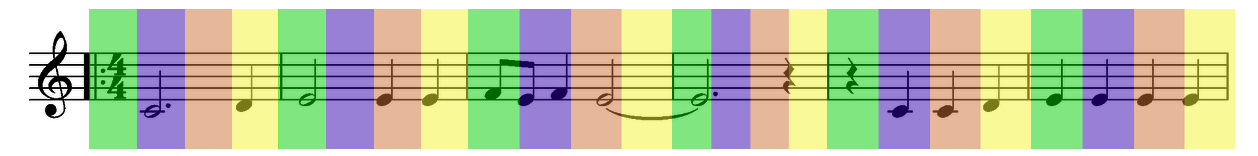
\includegraphics[width=1\textwidth]{./imagenes/sincronotas}
\caption{Sincronización en cada pulso a un músico diferente} \label{fig:sincronotas}
\end{figure}

En la figura \ref{fig:sincronotas} se está sincronizando a un músico por pulso. En
la figura del ejemplo habría cuatro músicos (por eso hay cuatro colores).\\

Al sincronizarse a un músico en cada pulso y que él mantenga el mismo tempo que los demás,
la sincronización no se pierde (salvo que, por algún motivo), una recepción tarde más de
la cuenta.\\

Esto tal vez haga que la red tenga demasiadas tareas y la fiabilidad disminuya. Para
cubrir este aspecto, no se sincroniza en cada pulso, si no en cada compás (como hay
cuatro pulsos en cada compás, las comunicaciones se reducen a una cuarta parte).
En la figura \ref{fig:sincrocompas} se puede ver de forma gráfica.\\

\begin{figure}[!htb]
\centering
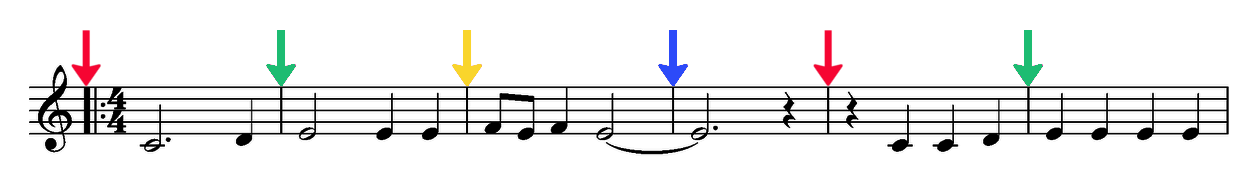
\includegraphics[width=1\textwidth]{./imagenes/sincrocompas}
\caption{Sincronización en cada compás a un músico diferente} \label{fig:sincrocompas}
\end{figure}

Cada flecha de un color es un músico sincronizado. Al igual que en el ejemplo anterior,
deberá mantener el tempo de forma local, hasta que llegue otra señal por parte del director.\\

Que el director envíe constantemente el pulso permite que, en caso que uno de los
paquetes haya llegado más tarde de la cuenta, se pueda corregir.\\

Para comprobar que funciona, se hace un experimento similar al de los casos anteriores pero,
esta vez, midiendo tiempos en dos dispositivos receptores.

\begin{figure}[!htb]
\centering
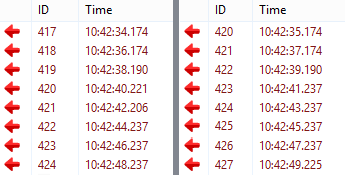
\includegraphics[width=0.7\textwidth]{./imagenes/sincronizacion}
\caption{Sincronización en cada compás a un músico diferente} \label{fig:sincronizacion}
\end{figure}



  \begin{figure}[!htb]
  \centering
  \captionsetup{justification=centering}
  \resizebox{0.9\textwidth}{!}{
  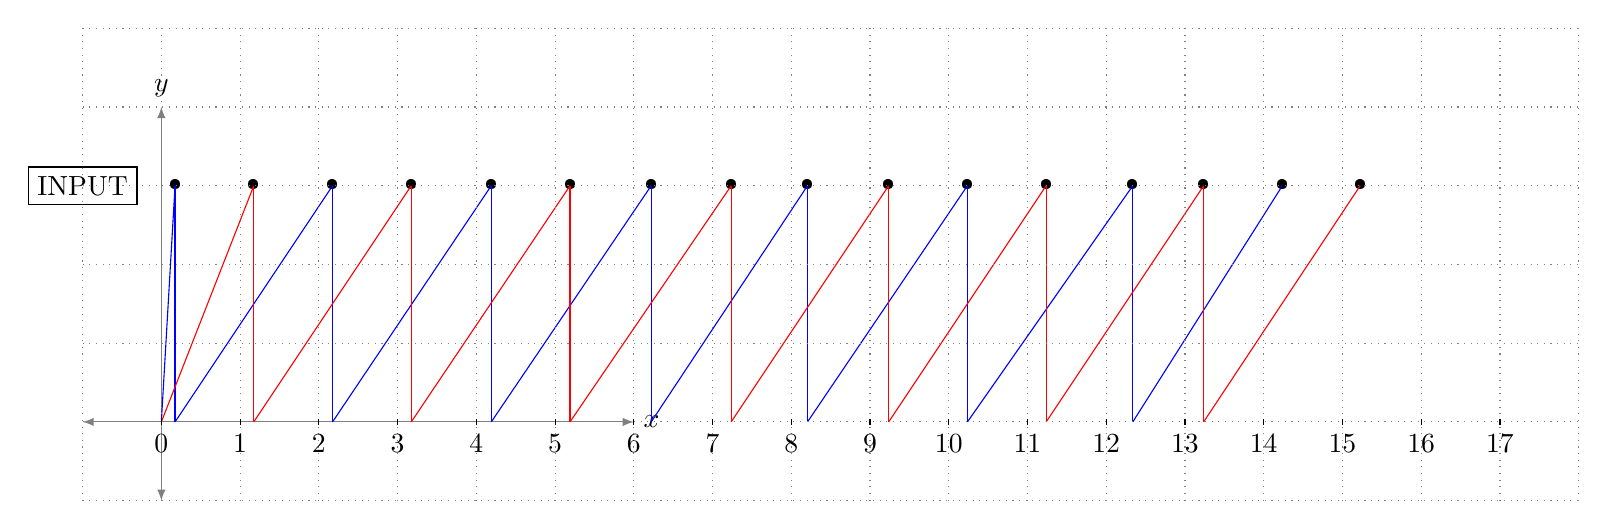
\begin{tikzpicture}
  \draw[latex-latex, thin, draw=gray] (-1,0)--(6,0) node [right] {$x$};
  \draw[latex-latex, thin, draw=gray] (0,-1)--(0,4) node [above] {$y$};


%Primero el izquierdo
  \foreach \Point in {(0.174,3),(2.174,3),(4.190,3),(6.221,3),(8.206,3),(10.237,3),
  (12.337,3),(14.237,3)}{
     \node at \Point {\textbullet};
  }

  \draw [blue,solid] (0,0) -- (0.174,3);
  \draw [blue,solid]  (0.174,3) -- (0.174,0);
  \draw [blue,solid]  (0.174,0) -- (2.174,3);
  \draw [blue,solid]  (2.174,3) -- (2.174,0);
  \draw [blue,solid]  (2.174,0) -- (4.190,3);
  \draw [blue,solid]  (4.190,3) -- (4.190,0);
  \draw [blue,solid]  (4.190,0) -- (6.221,3);
  \draw [blue,solid]  (6.221,3) -- (6.221,0);
  \draw [blue,solid]  (6.221,0) -- (8.206,3);
  \draw [blue,solid]  (8.206,3) -- (8.206,0);
  \draw [blue,solid]  (8.206,0) -- (10.237,3);
  \draw [blue,solid]  (10.237,3) -- (10.237,0);
  \draw [blue,solid]  (10.237,0) -- (12.337,3);
  \draw [blue,solid]  (12.337,3) -- (12.337,0);
  \draw [blue,solid]  (12.337,0) -- (14.237,3);

%Ahora el derecho
\foreach \Point in {(1.174,3),(3.174,3),(5.190,3),(7.237,3),(9.237,3),(11.237,3),(13.237,3),(15.225,3)}{
   \node at \Point {\textbullet};
}

\draw [red,solid] (0,0) -- (1.174,3);
\draw [red,solid] (1.174,3) -- (1.174,0);
\draw [red,solid] (1.174,0) -- (3.174,3);
\draw [red,solid] (3.174,3) -- (3.174,0);
\draw [red,solid] (3.174,0) -- (5.190,3);
\draw [red,solid] (5.190,3) -- (5.190,0);
\draw [red,solid] (5.190,0) -- (7.237,3);
\draw [red,solid] (7.237,3) -- (7.237,0);
\draw [red,solid] (7.237,0) -- (9.237,3);
\draw [red,solid] (9.237,3) -- (9.237,0);
\draw [red,solid] (9.237,0) -- (11.237,3);
\draw [red,solid] (11.237,3) -- (11.237,0);
\draw [red,solid] (11.237,0) -- (13.237,3);
\draw [red,solid] (13.237,3) -- (13.237,0);
\draw [red,solid] (13.237,0) -- (15.225,3);


  \draw [dotted, gray] (-1,-1) grid (18,5);

  \foreach \x in {0,1,2,3,4,5,6,7,8,9,10,11,12,13,14,15,16,17}
      \draw (\x cm,1pt) -- (\x cm,-1pt) node[anchor=north] {$\x$};

  \node[draw] at (-1,3) {INPUT};
  \end{tikzpicture}
  }


  \caption{Representación temporal de la llegada de paquetes utilizando \textit{unicast}\\
  (X está en segundos)} \label{fig:graficasincronizados}
  \end{figure}

Como se puede ver en \ref{fig:sincronizacion} y \ref{fig:graficasincronizados},
la sincronización que se ha obtenido es bastante buena. Cada uno de los dispositivos
es sincronizado cada un segundo (por eso, si miramos una de las trazas,
vemos que hay en torno a dos segundo de espera entre la llegada de un paquete y otro
-1 segundo para sincronizar al otro XBee y 1 para sincronizar al que estamos monitorizando-).\\

Si examinamos las trazas, se observa cómo hay, en algunas ocasiones, sincronización
a nivel de milisegundos. También es interesante ver que en muchas ocasiones (como en los
paquetes de la traza de la derecha con ID comprendidas entre 423 y 426 -inclusive-) la
llegada de paquetes es en el mismo milisegundo de segundos distintos, por ejemplo: en el
momento 10:42:45.237 (ID:425) y 10:42:47.237 (ID:426). Cuando esto no ocurre, el error es asumible.\\



\section{Modalidades del dispositivo}
\title{Modalidades del dispositivo}

Tras el análisis realizado sobre la estructura de la red, toca hablar de los dos tipos
de nodos de los que se disponen: director y músico.

\subsection{Dispositivo director}
\title{Dispositivo director}

El dispositivo del director tiene que comunicarse con el resto de dispositivos (los
de los músicos) y con el dispositivo Android. Para enlazar con los otros músicos
se va a utilizar la red inalámbrica de sensores mientras que, para la conexión
con el dispositivo Android se ha elegido utilizar Bluetooth (HC05 \cite{bthc05}) ya que es un sistema
de comunicación que tienen todos los dispositivos móviles (tanto \textit{tablets} como
\textit{smartphones}). Además (ya se estudió al principio de este capítulo), la versión
4 de Bluetooth tiene mecanismos para ahorro de energía (y como la comunicación va a durar
poco tiempo, no se necesita más).\\


\subsection{Configuración de la mota director}
\title{Configuración de la mota director}
\label{sec:configuracionmotadirector}

En la sección \ref{xctu} se vió un poco sobre la interfaz de XCTU. Ahora vamos a ver cómo
configurar una mota (para ser más exactos, la mota ``director").\\

En primer lugar será necesario descubrir la mota que tengamos conectada a nuestro ordenador
(como se dijo en \ref{xctu}, en la parte superior izquierda se utiliza cualquiera de las dos
opciones para buscar la mota). Después, accedemos al panel de configuración de la derecha y
seleccionamos ``Update firmware" (figura \ref{fig:configurar_mota_1}).

\begin{figure}[!htb]
\centering

\includegraphics[width=1\textwidth]{./imagenes/configurar_mota_1}
\caption{Subpanel dentro de la configuración} \label{fig:configurar_mota_1}
\end{figure}

Seleccionaremos el firmware que queramos instalar y hacemos click en ``Update".
En nuestro caso vamos a instalar ``ZigBee coordinator API", ya que estamos
configurando la mota del director.

\begin{figure}[!htb]
\centering

\includegraphics[width=1\textwidth]{./imagenes/configurar_mota_1}
\caption{Subpanel dentro de la configuración} \label{fig:configurar_mota_2}
\end{figure}

Cuando la instalación finalice, haremos click sobre la restauración de valores de fábrica
(es el botón que se encuenta a la izquierda de la actualización de firmware en la figura \ref{fig:configurar_mota_1}).\\

Ahora solo faltará insertar un PAN ID, cambiar el modo API a 2, desactivar los pines (D0, D1, D2, D3, D4, D5, P1 y P2
-para que no consuman recursos-) y escribir los cambios en nuestro XBee.\\


\subsection{Controlador del dispositivo director}
\title{Controlador del dispositivo director}

Para llevar a cabo todo el proceso que se ha ido describiendo, es necesario programar
la placa Arduino. Teniendo en cuenta que hay que cumplir unos requisitos de tiempo bastante
fuertes, se ha elegido trabajar con timers. Arduino cuenta con dos timers: uno reservado
a la ejecución del propio código y otro que puede ser utilizado por el desarrollador.
La biblioteca ``Timer1" \cite{timeronearduino} facilita la manipulación de esta característica.\\

Por otra parte, es necesaria la utilización de dos puertos serial (uno pra XBee y otro para el Bluetooth).
La mayoría de versiones de Arduino (Lilypad, por ejemplo), no tienen más de un puerto.
Por ello se utiliza la biblioteca ``Software Serial" \cite{softwareserial} que, mediante software, consigue
que unos puertos que no son puerto serial, actúen como tal.\\

A continuación se muestra un pseudocódigo de lo que se ha implementado.
\floatname{algorithm}{Algoritmo}
\begin{algorithm}
  \begin{algorithmic}[1]
     \State $tiempo\gets 0$
     \State $i\gets 0$
     \State $leer \gets true$\\

     \Function{Envio}{}
      \If {$ahora - tiempo\geq periodo $}
        \State enviarPaquete($i$)
        \State $i \gets i+1(mod(numeroXBee))$
        \State $tiempo \gets ahora$
      \EndIf
      \EndFunction\\

    \While{true}
    \If{$leer$}
      \If{Hay datos del Bluetooth}
        \State $leer \gets false$
        \State $periodo\gets tiempoEntrePulso(leerBluetooth())*4$
        \State Se generan los paquetes
        \State Se inicia el timer con la funcion Envio
      \EndIf
     \EndIf
    \EndWhile
  \end{algorithmic}
  \caption{Algoritmo utilizando por el controlador del director}
\end{algorithm}

  \begin{enumerate}
  \item Se declara la función que ejecutará el timer. Esta función comprueba cuánto
   tiempo ha pasado desde la última vez que se ejecutó
    \begin{itemize}
      \item Si ha pasado suficiente, enviará un mensaje al nodo que le toque sincronizar
    \end{itemize}
  \item En el bucle que se ejecuta continuamente, si leer(*) es verdadero:
    \begin{enumerate}
      \item Se lee del Bluetooth el tempo y se generan los paquetes para cada dirección XBee
      \item Se calculan los pulsos por segundo, después el tiempo entre pulso y se multiplica
      por 4 (para sincronizar cada 4 pulsos, es decir, cada compás de 4/4)
      \item Se generan los paquetes a enviar
      \item Se activa el timer (cada medio milisegundo para mantenerlo en activo -aunque haya momentos que se llame
      al timer para nada, esto provoca que sea más preciso que si lo ajustásemos al tiempo entre pulsos y, de todas formas,
      va a quedar en el bucle de espera activa, la función ``loop"-).
    \end{enumerate}
\end{enumerate}

Lo que se acaba de explicar es el algoritmo. En la implementación en Arduino, se necesitan
declarar los pines, inicializar algunas variables... También se desactiva el Bluetooth para
ahorrar energía.\\

Cuando se ha enviado un paquete a cada dispositivo, se vuelve a empezar (por eso se aplica la función módulo).\\

(*)Esta variable ``leer"\ permite que, una vez que se apaga el Bluetooth, no se vuelva a intentar leer
(ya que no se conseguirán datos -y la lectura de serial es más lenta- o estos serán erróneos
-lo que nos llevará a un fallo en el sistema-).\\


\subsection{Esquema de conexionado del dispositivo director}
\title{Esquema de conexionado del dispositivo director}

Este esquema se puede consultar en la figura \ref{fig:director_esquema}. Falta
la mota XBee, que iría sobre la shield, y la alimentación que se realizaría mediante un
dispositivo FTDI-USB (ambos no se han incluido para que sea más sencilla la lectura del
esquema).\\

Para realizar las pruebas se ha utilizado un Arduino UNO por falta de material aunque,
como se muestra en la figura \ref{fig:director_esquema}, lo deseado es utilizar la
versión \textit{wearable} de Arduino.

\begin{figure}[!htb]
\centering
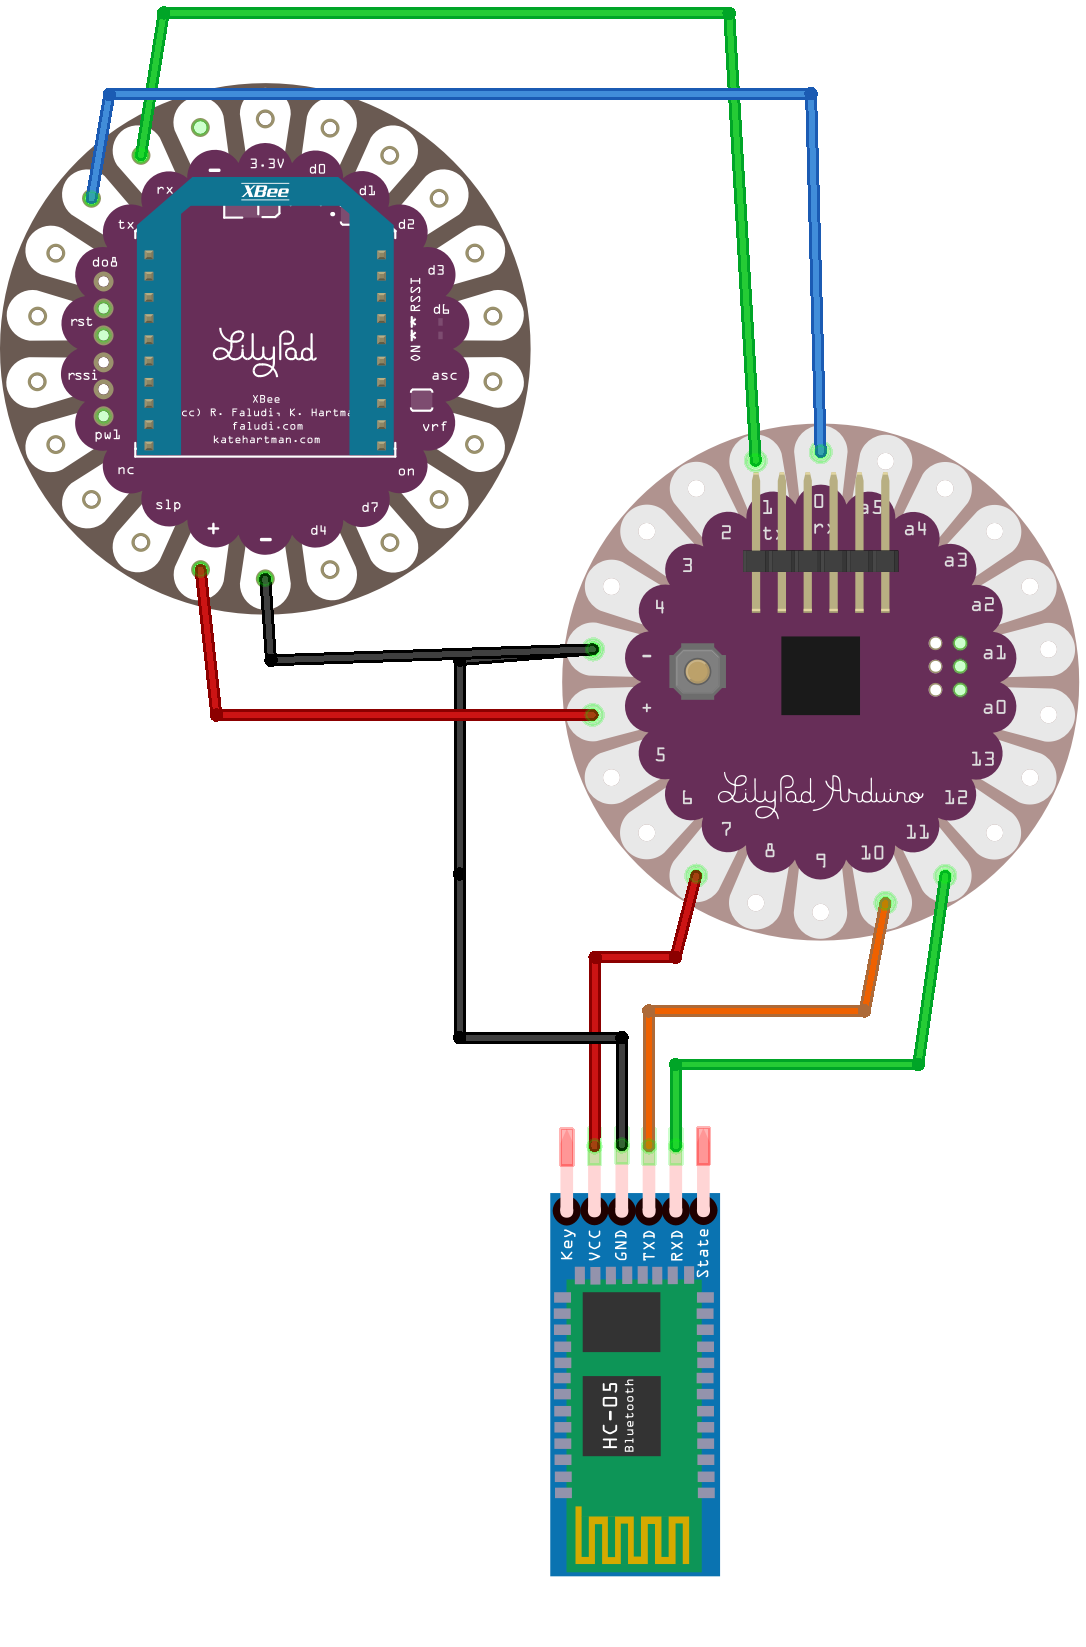
\includegraphics[width=1\textwidth]{./imagenes/director_esquema}
\caption{Esquema de conexionado del director} \label{fig:director_esquema}
\end{figure}

\clearpage

\subsection{Carcasa del dispositivo director}
\title{Carcasa del dispositivo director}

\begin{figure}[!htb]
\centering
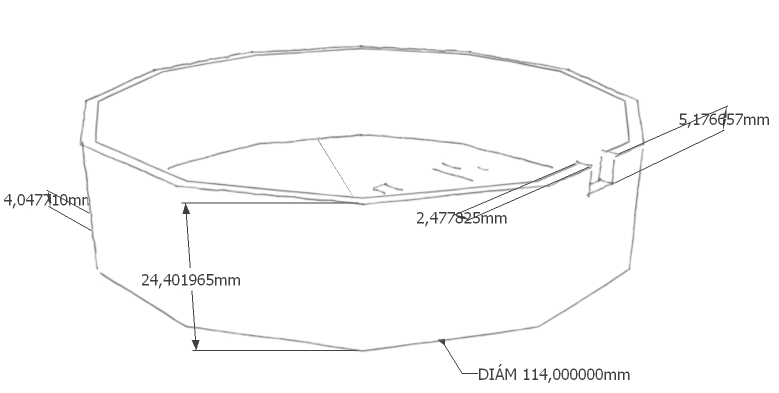
\includegraphics[width=1\textwidth]{./imagenes/carcasa_base_director}
\caption{Base de la carcasa para el director} \label{fig:carcasa_base_director}
\end{figure}

\begin{figure}[!htb]
\centering
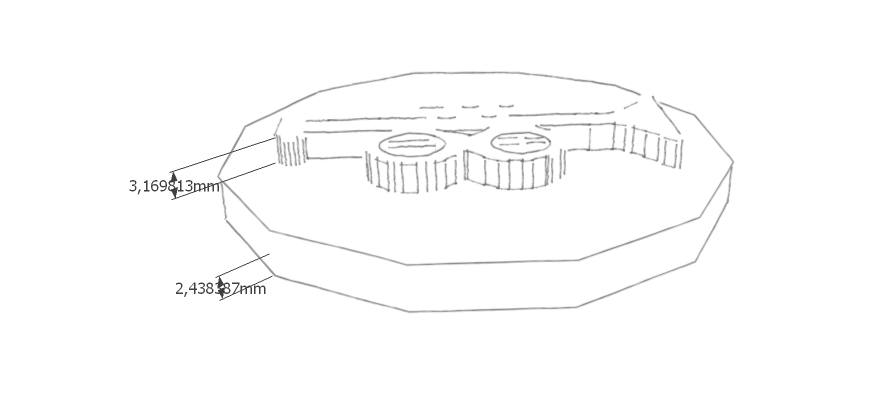
\includegraphics[width=1\textwidth]{./imagenes/carcasa_tapa}
\caption{Tapa de la carcasa} \label{fig:carcasa_tapa}
\end{figure}

\begin{figure}[!htb]
\centering
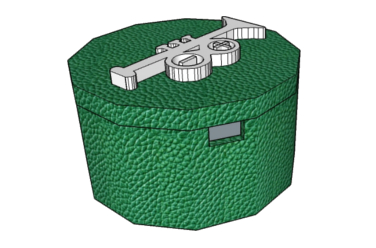
\includegraphics[width=0.5\textwidth]{./imagenes/carcasa_modelo_director}
\caption{Modelo 3D de la carcasa} \label{fig:carcasa_modelo}
\end{figure}


\begin{figure}[!htb]
\centering

\includegraphics[width=0.5\textwidth]{./imagenes/carcasa_modelo_director_abajo}
\caption{Modelo 3D de la carcasa visto desde la parte inferior} \label{fig:carcasa_inferior}
\end{figure}

La carcasa que se propone tiene dos partes:
\begin{itemize}
  \item Base: dentro de esta parte van todos los componentes. En la parte inferior pone ``Director"
  para poder diferenciarlo de los dispositivos de los músicos
  \item Tapa: permite dejar todos los componentes dentro para que no se salgan. LLeva el logotipo
  de ArduBand. Se une a la base utilizando algún adhesivo.
\end{itemize}

El hueco que queda libre es para colocar ahí la salida a MiniUSB del FTDI (para conectar la alimentación).\\

\subsection{Dispositivo músico}
\title{Dispositivo músico}

Solamente necesita comunicarse con el director (a través de la \textit{WSN}). Por otro lado,
también hay que marcar el pulso al músico (con el micromotor de la figura \ref{fig:micromotor}).

\subsection{Configuración de la mota músico}
\title{Configuración de la mota músico}

La configuración es igual que en el caso de la mota director (como se hizo en la sección
\ref{sec:configuracionmotadirector}). Lo que cambia es el firmware que se instala, que es el
``ZigBee End Device API".

Hay que insertar la misma PAN ID que insertásemos en el director o nuestros dispositivos
no podrán comunicarse.\\

En función del número de músicos de los que dispongamos, podremos hacer una estimación de
cuánto tiempo máximo se tardará en sincronizarlos y, en función de eso,
establecer un tiempo para que las motas puedan activar el estado de ahorro energético.
Es decir, si se sobrepasa el tiempo en el que el director debería haber enviado una
nueva señal, enviar a ``dormir" las motas, de forma que consman menos energía.


\subsection{Controlador del dispositivo músico}
\title{Controlador del dispositivo músico}
Al igual que en el caso del director, se necesita cumplir unos requisitos de tiempo
bastante fuertes:
\begin{itemize}
  \item La lectura de los datos recibidos por XBee debe hacerse rápidamente
  \item El pulso debe mantenerse de manera local (con el mínimo error posible)
\end{itemize}

Es de vital importancia que todos lo dispositivos de los músicos estén controlados
por Arduino que midan el tiempo de igual forma. Es decir, que los \textit{delay,
timers} y similares funciones midan la misma cantidad de tiempo. Para explicarlo
mejor se pone el siguiente ejemplo:\\
supongamos que tenemos dos Arduino ( ya sean del mismo fabricante o de otro). Si en ambos dispositivos
cargamos el ejemplo de \textit{blink} \cite{arduinoBlink} (es un ejemplo que viene
en el IDE de Arduino y que permite controlar un led, manteniéndolo encendido durante un segundo
y dejándolo apagado durante otro), ambos deben mantener la misma cantidad de tiempo
el led encendido y/o apagado.\\

La afirmación del anterior párrafo parece algo que se deba cumplir, al menos, entre
Arduino de la misma clase (UNO y derivados, Leonardo y derivados...), pero no es así.
Tras un experimento con un Arduino UNO (oficial) y una placa DCcduino (compatible con UNO),
se pudo comprobar que, mientras Arduino UNO se mantenía constante, la placa DCcduino iba a una
mayor velocidad (en vez de cambiar de estado de encendido a apagado o de apagado a encendido
cada un segundo, lo hacía a un tiempo sensiblemente menor). Ambas placas se anuncian
con una velocidad de reloj de 16MHz (el lector puede consultar en \cite{arduinoUNO} las
especificaciones de la placa Arduino UNO mientras que, para la placa DCcduino, no ha sido
posible encontrar unas especificaciones propias ya que todas las páginas hacen referencia
a las de Arduino UNO), algo que parece no ser cierto.\\

Si todos los músicos no tienen el mismo modelo de \textit{timer} (o uno que mida igual),
la subdivisión que se proponía al final de la subsección \ref{subsec:problemabroadcast},
no funcionará.\\

\floatname{algorithm}{Algoritmo}
\begin{algorithm}
  \begin{algorithmic}[1]
    \State $periodo\gets 500$
    \State $tiempo\gets 0$

    \Function{Vibrar}{}
     \If {$ahora - tiempo \geq periodo$}
       \State activaActuador()
       \State $tiempo \gets ahora$
      \Else \If{$ahora - tiempo \geq 300$}
        \State desactivaActuador()
         \EndIf
     \EndIf
     \EndFunction\\

     \State Se\ inicia\ el\ timer\ con\ la\ función Vibrar

     \While{true}
     \If{$datosXBee$}
         \State $periodo\gets tiempoEntrePulso(leerXBee())$
      \EndIf
     \EndWhile
  \end{algorithmic}
  \caption{Algoritmo utilizando por el controlador del músico}
\end{algorithm}

\begin{enumerate}
  \item Se inicia a un periodo de 2000 ms (simplemente para que el actuador pueda comenzar a
  funcionar)
  \item Se inicializa el tiempo
  \item Se declara la función Vibrar
    \begin{itemize}
      \item Si ha pasado suficiente tiempo para activar el actuador
        \begin{enumerate}
          \item Activar actuador
          \item Se guarda el momento en el que se activó
        \end{enumerate}
      \item Si ha pasado suficiente tiempo para desactivarlo(*), se desactiva
    \end{itemize}
  \item Se inicia el timer
  \item En el bucle
    \begin{enumerate}
      \item Lectura del tempo
      \item Cálculo del tiempo entre pulsos
    \end{enumerate}
\end{enumerate}

(*) Este tiempo se ha calculado de forma empírica. Si se inserta un tiempo superior,
cuando la velocidad de interpretación es de alrededor de los 120 pulsos por minuto,
el actuador permanece activo siempre (por lo que no se marca el pulso). Para un tiempo
menor, la vibración puede no ser suficiente o, incluso, el actuador podría no llegar a
activarse.\\

Se ha utilizado un Arduino Lilypad compatible. Este derivado, es detectado por el IDE de Arduino
como una placa con una velocidad de 8MHz, sin embargo,
este derivado funciona a 16MHz (por lo que va al doble de rápido). Si, por ejemplo, pedimos que espere
1 segundo, esperará 500ms. También afecta al puerto serie: cuando se abre un puerto serial a una velocidad
de 4800bps, realmente se está abriendo a 9600bps (es por eso que en la implementación en Arduino, se han multiplicado
los tiempos por 2 y se ha abierto el puerto serie a una velocidad de 4800bps).\\

\subsection{Esquema de conexionado del dispositivo músico}
\title{Esquema de conexionado del dipositivo músico}

\begin{figure}[!htb]
\centering
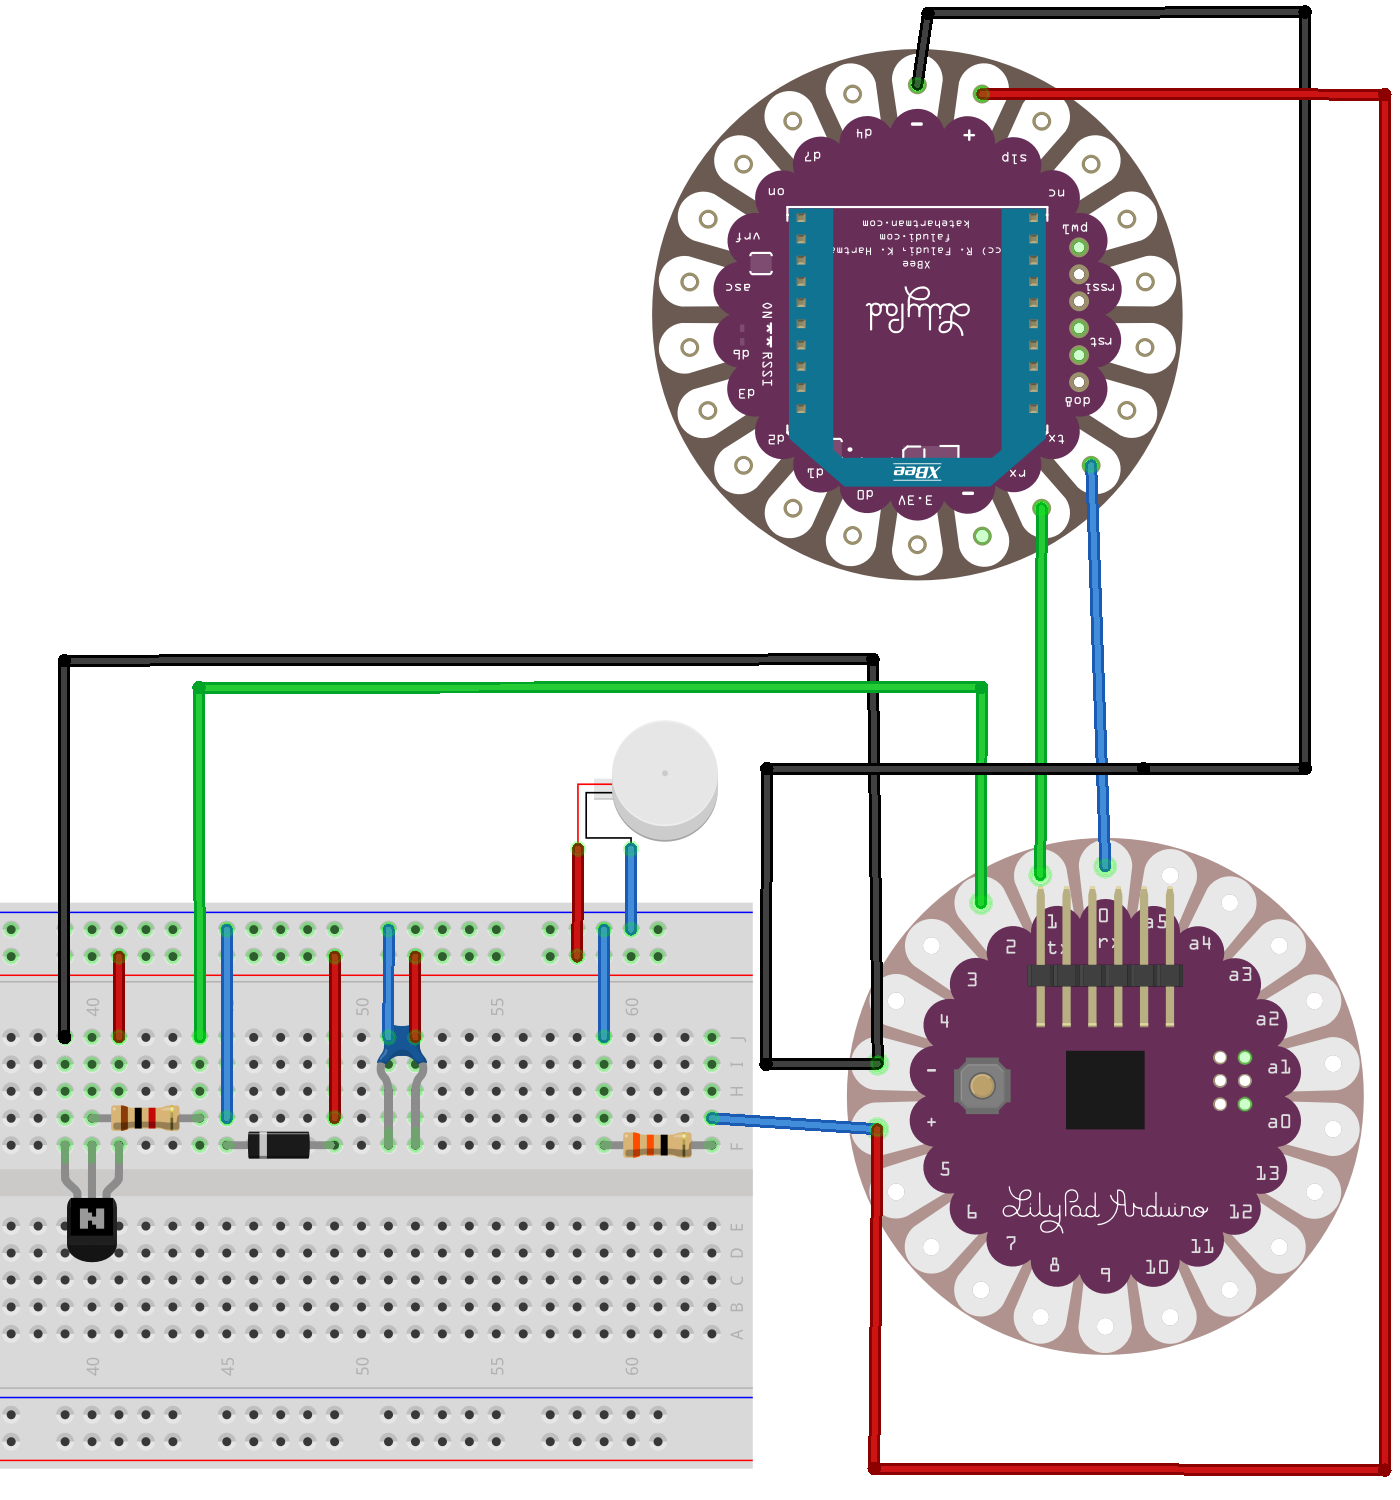
\includegraphics[width=1\textwidth]{./imagenes/musico_esquema}
\caption{Esquema de conexionado del músico} \label{fig:musico_esquema}
\end{figure}


\subsection{Carcasa del dispositivo músico}
\title{Carcasa del dispositivo músico}

También está compuesto por dos piezas:
\begin{itemize}
  \item Carcasa: es igual a la de la figura \ref{fig:carcasa_tapa}.
  \item Base: es similar a la del director pero tiene un menor tamaño (ya que el espacio
  de los componentes no es tan grande como el del dispositivo Bluetooth). En la base,
  de igual forma que está escrito ``Director" en el otro dispositivo, tiene escrito
  ``Músico".
\end{itemize}


\begin{figure}[!htb]
\centering
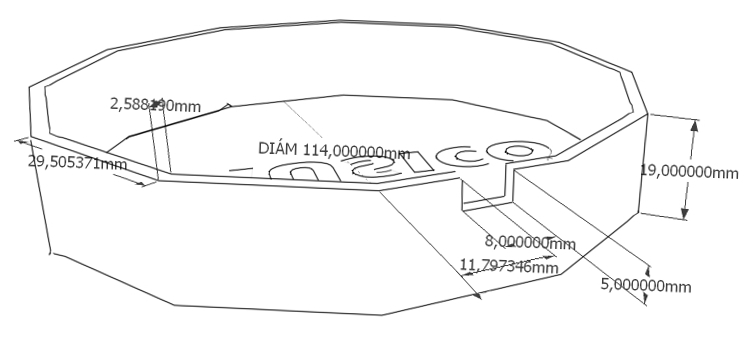
\includegraphics[width=1\textwidth]{./imagenes/carcasa_base_musico}
\caption{Base de la carcasa para el músico} \label{fig:carcasa_base_musico}
\end{figure}


\begin{figure}[!htb]
\centering
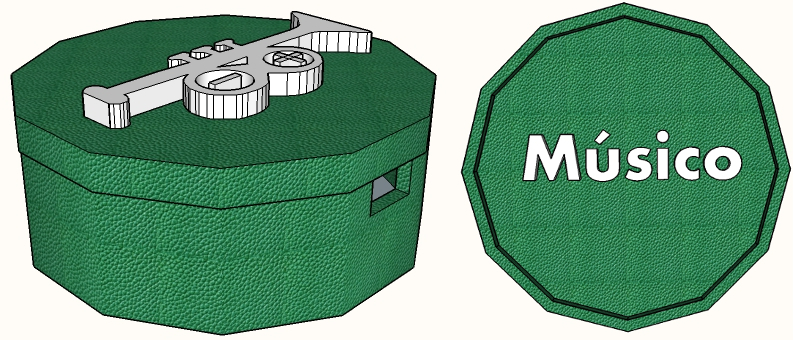
\includegraphics[width=0.6\textwidth]{./imagenes/carcasa_modelo_musico}
\caption{Modelo 3D de la carcasa del músico} \label{fig:carcasa_musico}
\end{figure}
